%
% Chapter 2
%

\chapter{Experimental Setup}
\label{chap:setup}

\section{Overview}

For E0 transitions, two types of radiation must be measured: conversion electrons and gamma rays. As conversion electron transitions and intensities are usually tabulated as conversion coefficients, which compare the electron intensities to the respective gamma-rays from the transition, both conversion electrons and gamma-rays must be measured in this experiment. Further, to identify pure E0 transitions, the experiment must show no corresponding gamma rays.

Due to the high level density of nuclei in the rare-earth region, detectors with high resolution are favored for these experiments. The detectors must also be placed in a way that allows for simultaneous measurement of both particles and gamma-rays. For good resolution, high purity germanium (HPGe) detectors are the standard for gamma-rays. For electron detection, silicon-based detectors have the best resolution. The electron energies of interest range from less than 100 keV to over 1 MeV. Standard silicon detectors do not have an energy range that high for electrons, so lithium-drifted silicon (Si(Li)) detectors were used, which have a higher top-end electron energy sensitivity.

To make these measurements, three separate experiments were performed at the Nuclear Science Laboratory (NSL) at the University of Notre Dame using the Internal Conversion Electron Ball (ICEBall) Spectrometer paired with two configurations of HPGe detectors: GEORGINA and Clovershare (Figure \ref{fig:clovershare_config}). 

%\begin{figure}
    \centering
    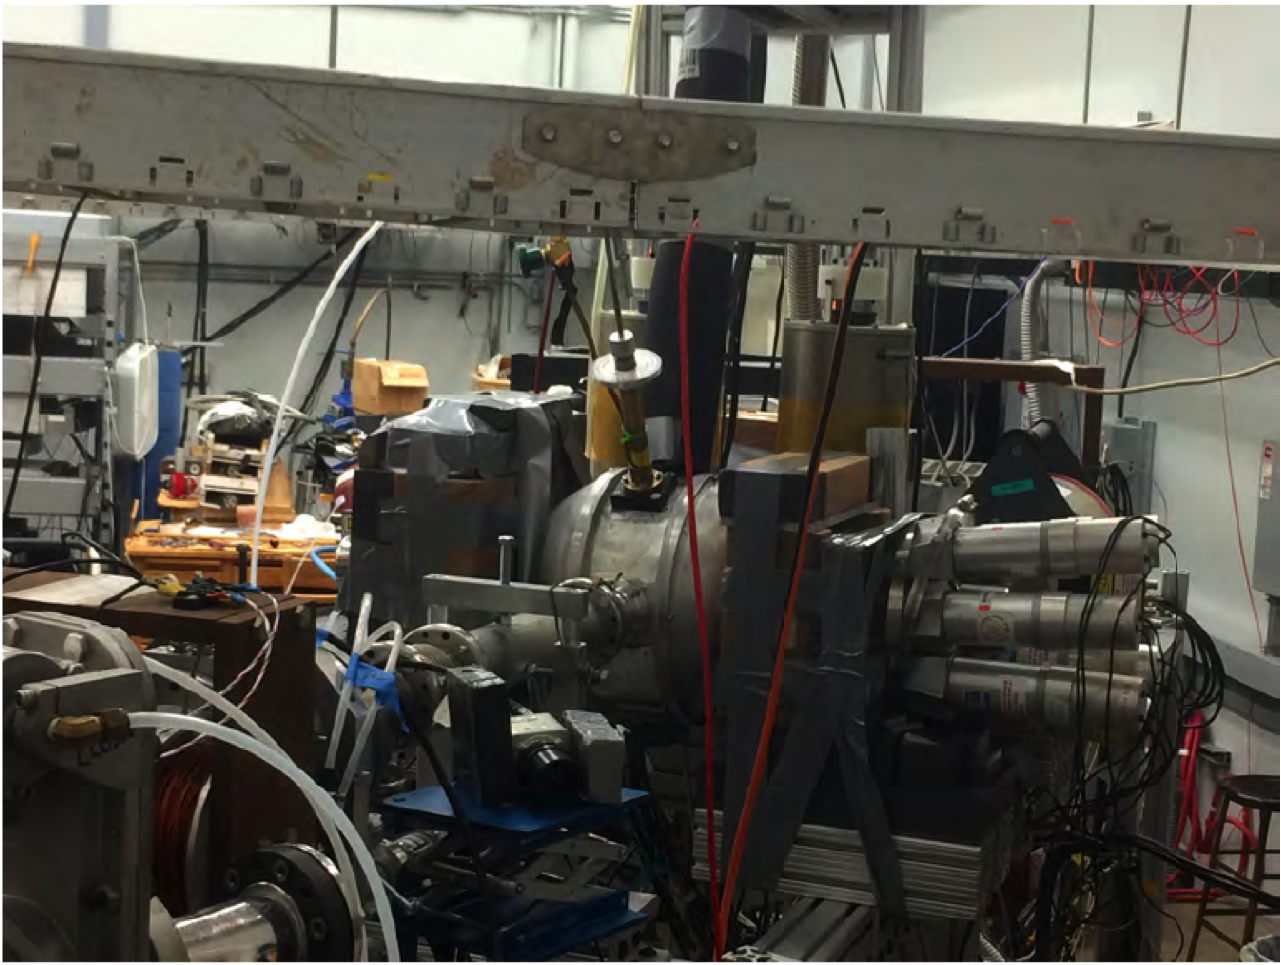
\includegraphics[scale=0.6]{Setup_Figs/ICEBall-2014.png}
    \caption{Image of the assembled experimental configuration with GEORGINA. One HPGe detector has BGO crystals around it.}
    \label{fig:georgina_config}
\end{figure}

\begin{figure}
    \centering
    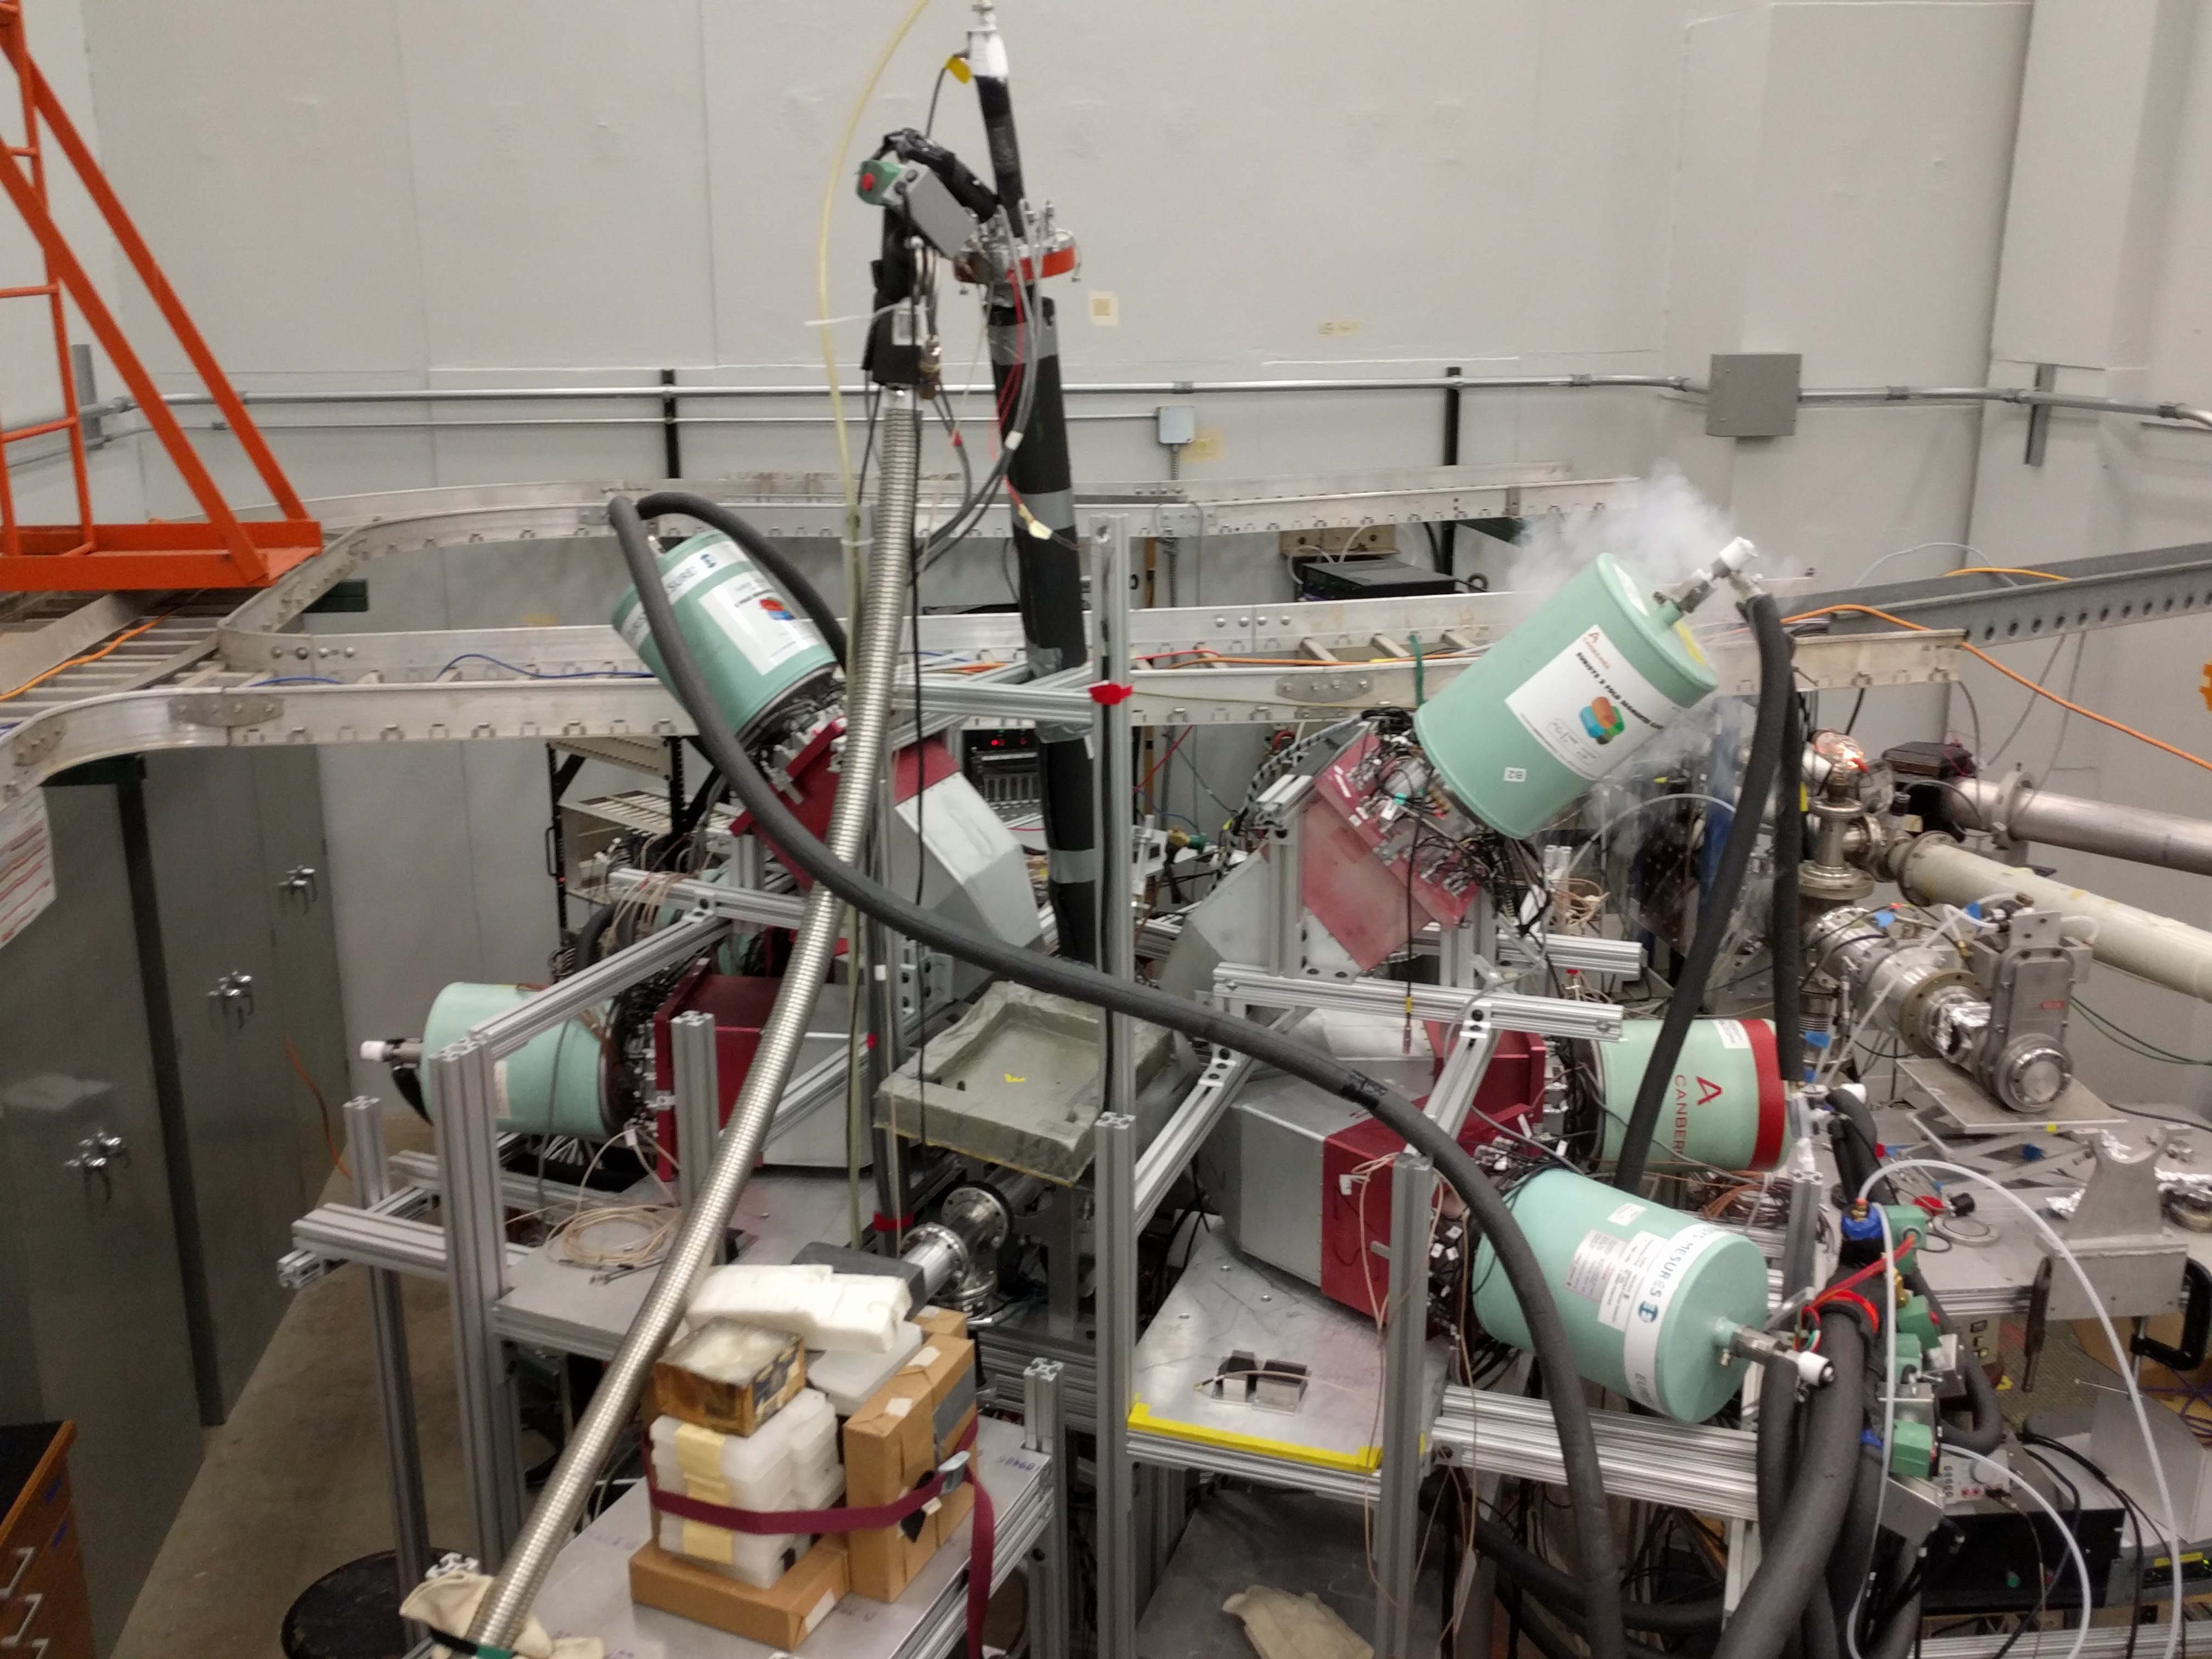
\includegraphics[scale=0.1]{Setup_Figs/IMG_20160311_192243.jpg}
    \caption{Image of the assembled experimental configuration with Clovershare. One HPGe detector is not visible from this angle.}
    \label{fig:clovershare_config}
\end{figure}

The $(\alpha,2n)$ reaction favors populating states of low, even-$J$ and positive parity. These states, including the $0^+$ states, are the ones of interest in this study, making this a natural reaction to select for the experiment. The $Q$ value for this reaction is -14.774 MeV for $^{154}$Gd and -13.638 MeV for $^{156}$Gd, meaning an alpha beam of the necessary energy for the reaction to occur is well within the capability of the NSL.

A Sm$(\alpha,2n)$Gd reaction was used with different enriched targets to create the desired Gd isotope, with an $\alpha$ beam of 20 MeV. A bunched beam was used to create timing for coincidence identification. This beam energy was determined by a measurement using a natural Sm target, with ICEBall and two neutron detectors. TALYS Nuclear Reaction Simulator was run to determine a range of energies to maximize the cross section of the desired reaction, while minimizing the neutron flux, as neutrons can damage HPGe detectors. Figure \ref{fig:alpha-neutron} shows the cross sections for the $(\alpha,xn)$ reactions for $^{154}$Sm in the $\alpha$ energy range of interest. Beam energies from 16 MeV to 21 MeV were tested. Measurements were done at 1 MeV intervals. The cross section was calculated using conversion electron measurements from ICEBall, and compared with the neutron flux at that energy.

\begin{figure}[t]
    \centering
    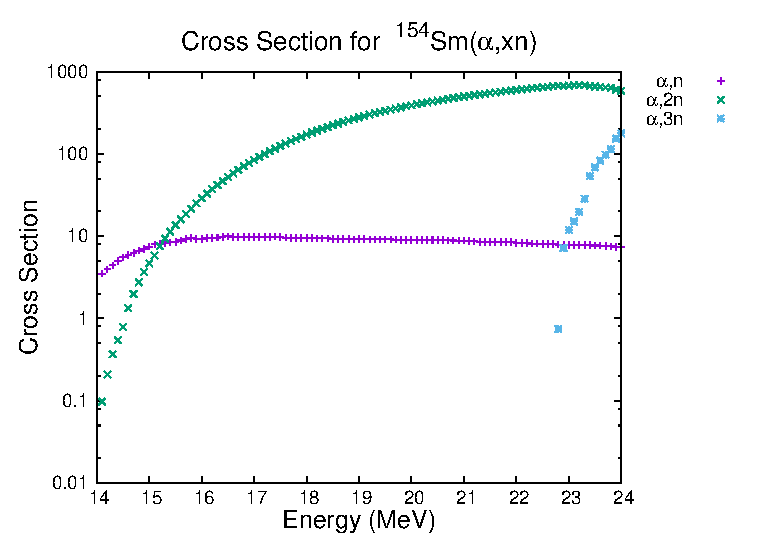
\includegraphics[scale=1]{Setup_Figs/alpha-n-comp.eps}
    \caption{Comparison between the cross sections of the $(\alpha,xn)$ reactions on $^{154}$Sm, calculated using Talys\citep{koning07:_talys}. The fewer neutrons being emitted, the lower the energy before the reaction occurs. Maximizing the cross section with respect to the neutron flux can be done by finding an energy where the desired reaction, $(\alpha,2n)$ can be maximized, while minimizing the $(\alpha,n)$ and $(\alpha,3n)$ reactions. Specifically, this means finding an energy before the $3n$ reaction has significant strength, while maximizing the $2n$ reaction, as the $n$ reaction is nearly the same across the energy regime of interest.}
    \label{fig:alpha-neutron}
\end{figure}

Two different forms of electronics were used for the data acquisition system. The data acquisition systems used were based on the NSCL DAQ\citep{nscl:_daq,prokop14:_nsclddas}. The electronics used with GEORGINA were shaped by NIM modules before going through ADC VME modules to the computer \citep{mesytec:_ADC,caen:_TDC}. The Clovershare data used the XIA Pixie-16 modules, which take the place of the NIM and VME modules for shaping and converting the signals to digital data \citep{xia:_pixie}.

The digital files were converted to files for the analysis software using \texttt{evt2root} \citep{smith14:_evt2root}. Analysis, reported in Chapter \ref{ch:analysis}, was done using the CERN Root Data Analysis Framework and Radware \citep{brun97:_root,radford00:_radware}.

\section{Nuclear Science Laboratory at Notre Dame}

Nuclear physics has been studied at the Nuclear Science Laboratory at the University of Notre Dame since 1934, with accelerators in operation since 1937. Currently, the NSL operates locally with three accelerators: the FN Tandem, the 5 MV Single-Ended Sta. Ana accelerator, and the 3 MV 9S Tandem. There is also a fourth accelerator, a 1 MV machine called CASPAR, located in the Homestake Mines in South Dakota. The experiments in this dissertation were performed on the FN Tandem. Figure \ref{fig:NSL} is the current layout of the NSL. The accelerator in the top right of the figure is the FN Tandem.

The FN Tandem has two ion sources: the Helium Ion Source (HIS) and the Multi-Cathode Source of Negative Ions Using Cesium Sputtering (MC-SNICS). Most elements can absorb the electrons donated from cesium to create negative ions. Helium cannot and needs a special source, as discussed below. For the experiments described, the HIS was used.

Due to the electron binding energy of helium, the HIS uses a duoplasmatron. Within the duoplasmatron, a thin tungsten wire is heated while surrounded by the source gas (helium). The tungsten wire emits electrons, and positively ionizes the helium. This helium is extracted from the duoplasmatron and focused by an einzel lens, where it then goes through the lithium charge exchange. This section of the HIS works as a small two stage acceleration system, although the charge exchange works by adding electrons instead of stripping them. The positively charged ions are accelerated through a lithium vapor, and some gain electrons, becoming neutral or negatively charged. Those ions that become negatively charged are accelerated out the other end of the HIS, before being sent to the FN Tandem. Figure \ref{fig:HIS} is a schematic of this system.

\begin{figure}[t]
    \centering
    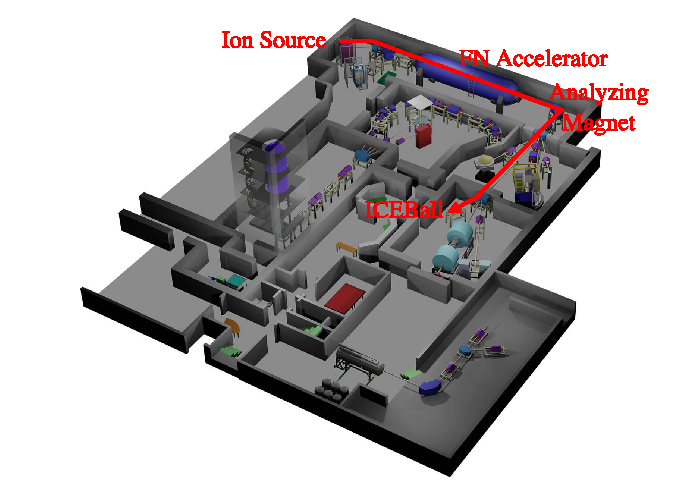
\includegraphics[scale=1.25]{Setup_Figs/NSL_2018_Layout.eps}
    \caption{Current layout of the Nuclear Science Laboratory at Notre Dame. The red line indicates the path taken by the beam, from ion source, through the accelerator and analyzing magnet, before being sent to ICEBall.}
    \label{fig:NSL}
\end{figure}

The FN Tandem has been in operation since 1968. Charging chains carrying a static charge deposit the charge on a terminal in the center of the machine. The charging chains are pelletron type, upgraded from the original insulated rubber belt system in 2000. The pelletron chain consists of metal pellets connected using nylon, allowing for each pellet to be electrically isolated as it carries electrical charge to the terminal \citep{nec:_pelletron}. The terminal is positively charged, and a pick-off system is used to remove electrons from the terminal shell, onto the pelletron chain. The beamline is kept at vacuum, but the area outside of the beamline and within the accelerator tank, is filled with a mixture of CO$_2$ and dry nitrogen gas, at approximately 200 PSI. To create a more uniform acceleration field, the terminal is brought to ground along the beamline using resistor-lined tubes. The resistors create a uniform electrical field down the tube, allowing for uniform acceleration.

It is known as a tandem because the system is a two-stage acceleration. Negatively charged ions enter the system, accelerating toward a positively charged terminal shell. Inside of the shell, the ions go through carbon stripping foils 3 $\mu g/cm^2$ thick, becoming positively charged as electrons are pulled off. The ions then accelerate away from the terminal for the second stage. The total energy gained by the ions is the terminal voltage times the quantity of one plus the final charge state.

\begin{figure}
    \centering
    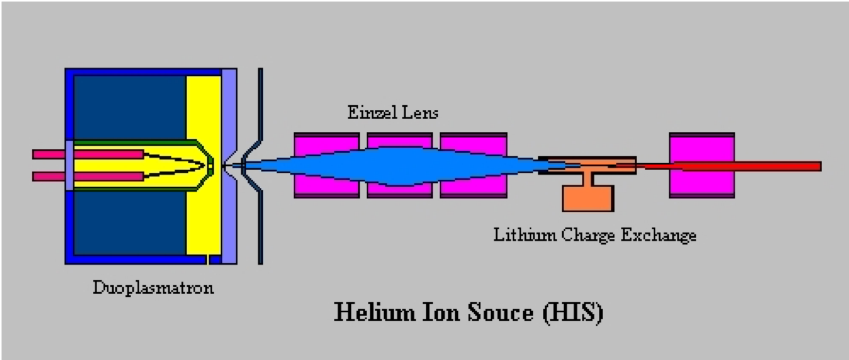
\includegraphics[scale=0.75]{Setup_Figs/HIS.png}
    \caption{A schematic of how the Helium Ion Source works.}
    \label{fig:HIS}
\end{figure}

After being sent through the accelerator, the beam goes through the analyzing magnet. This magnet is set for the specific species, energy, and charge state to bend 90 degrees to the experimental set ups.

\section{Beam Production}

Because of the use of HPGe detectors in an $(\alpha,2n)$ reaction, the neutron flux must be minimized in comparison to the cross section of the reaction, as the $(\alpha,n)$ reaction is also open. The neutrons being produced will interact with everything, including the HPGe detectors, which can be damaged by the $(n,\gamma)$ reaction on germanium. To do this minimization, a range of energies to test were selected by looking at theoretical cross sections in Talys\citep{koning07:_talys}. These energies were then tested with natural Sm targets, ICEBall, and two liquid scintillators to detect neutrons.

Samarium, as with many even-Z elements in the lanthanide region, has many stable isotopes. A total of five stable isotopes of Samarium exist, with two other isotopes being long-lived. Table \ref{tab:nat_Sm} summarizes the abundances and lifetimes of the various isotopes found in natural Samarium. The two isotopes used our enriched targets are the ones that have the highest natural abundances, $^{152,154}$Sm.

\begin{table}[]
    \centering
    \begin{tabular}{c|c|c}
    \toprule
         Isotope & Lifetime (y) & Abundance (\%)  \\
         \hline
         $^{144}$Sm & Stable & 3.08 \\
         $^{147}$Sm & $1.06\times10^{11}$ & 15.00 \\
         $^{148}$Sm & $7\times10^{15}$ & 11.25 \\
         $^{149}$Sm & Stable & 13.82 \\
         $^{150}$Sm & Stable & 7.37 \\
         $^{152}$Sm & Stable & 26.74 \\
         $^{154}$Sm & Stable & 22.74 \\
         \bottomrule
    \end{tabular}
    \caption{Isotope Distribution of Natural Samarium}
    \label{tab:nat_Sm}
\end{table}

\subsection{Talys Calculations}

Talys \citep{koning07:_talys} is code for simulation of nuclear reactions. Cross sections can be estimated using Talys to guide where an experimenter may want to run to optimize production, as is the case presently. 

Both natural and enriched Samarium targets were used and modelled within Talys. A range of energies, from 14 MeV to 24 MeV $\alpha$-particles were run. These energies allowed a large number of potential reaction products from elastic, inelastic, transfer, and knockout reactions. Figure \ref{fig:talys} is a visual summary of the strongest modelled reactions in the natural Samarium target. It was decided to test the energies between 16-21 MeV.

\begin{figure}[t]
    \centering
    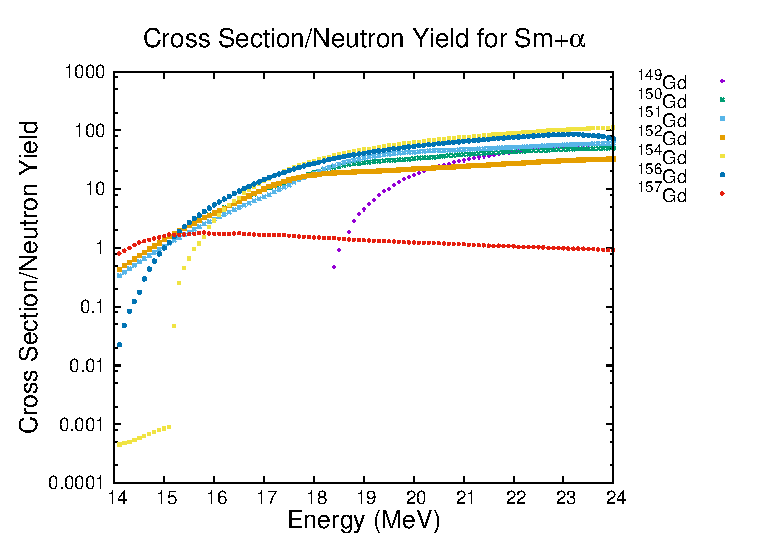
\includegraphics[scale=1]{Setup_Figs/Talys_Ratio.eps}
    \caption{Talys calculation of the highest cross sections divided by the total neutron yield in the natural Samarium target. Only the largest contributors are included, as there are a large number of products possible between the isotopes of Samarium in the target and the reactions channels open for each. All of the largest contributors are Gadolinium isotopes. The ratios for the isotopes of interest appear to plateau around 20-22 MeV.}
    \label{fig:talys}
\end{figure}

\subsection{Test Analysis and Results}

To test these Talys calculations and determine the best running energy, the cross section and neutron flux had to be measured at each energy without the use of the HPGe detectors. This was done using a natural Samarium target. ICEBall was used to measure the cross section by examining the K-electrons from ground-state band transitions in the reactions of interest, as the ground-state band is the most significantly populated band in the reaction. The DAQ described in Section \ref{sec:GEORGINA_electronics} was used. Spectra from ICEBall (described in Section \ref{sec:iceball})were fit using the methods described in Section \ref{sec:fitting}. The peaks were identified under the assumption the ground-state band transitions would be the strongest peaks in the spectra, and populate quickly. 

The neutrons were measured using two NE213 liquid organic scintillators. In these detectors, it is possible to do pulse shape discrimination, as the neutrons have longer decay times than the gammas in these detectors due to the nature of the interaction with the scintillating liquid \citep{knoll00:rad_det_meas}. This produces longer trails in the detectors, leading to different decay shapes, see Figure \ref{fig:pulse_discrimination}. 

\begin{figure}
    \centering
    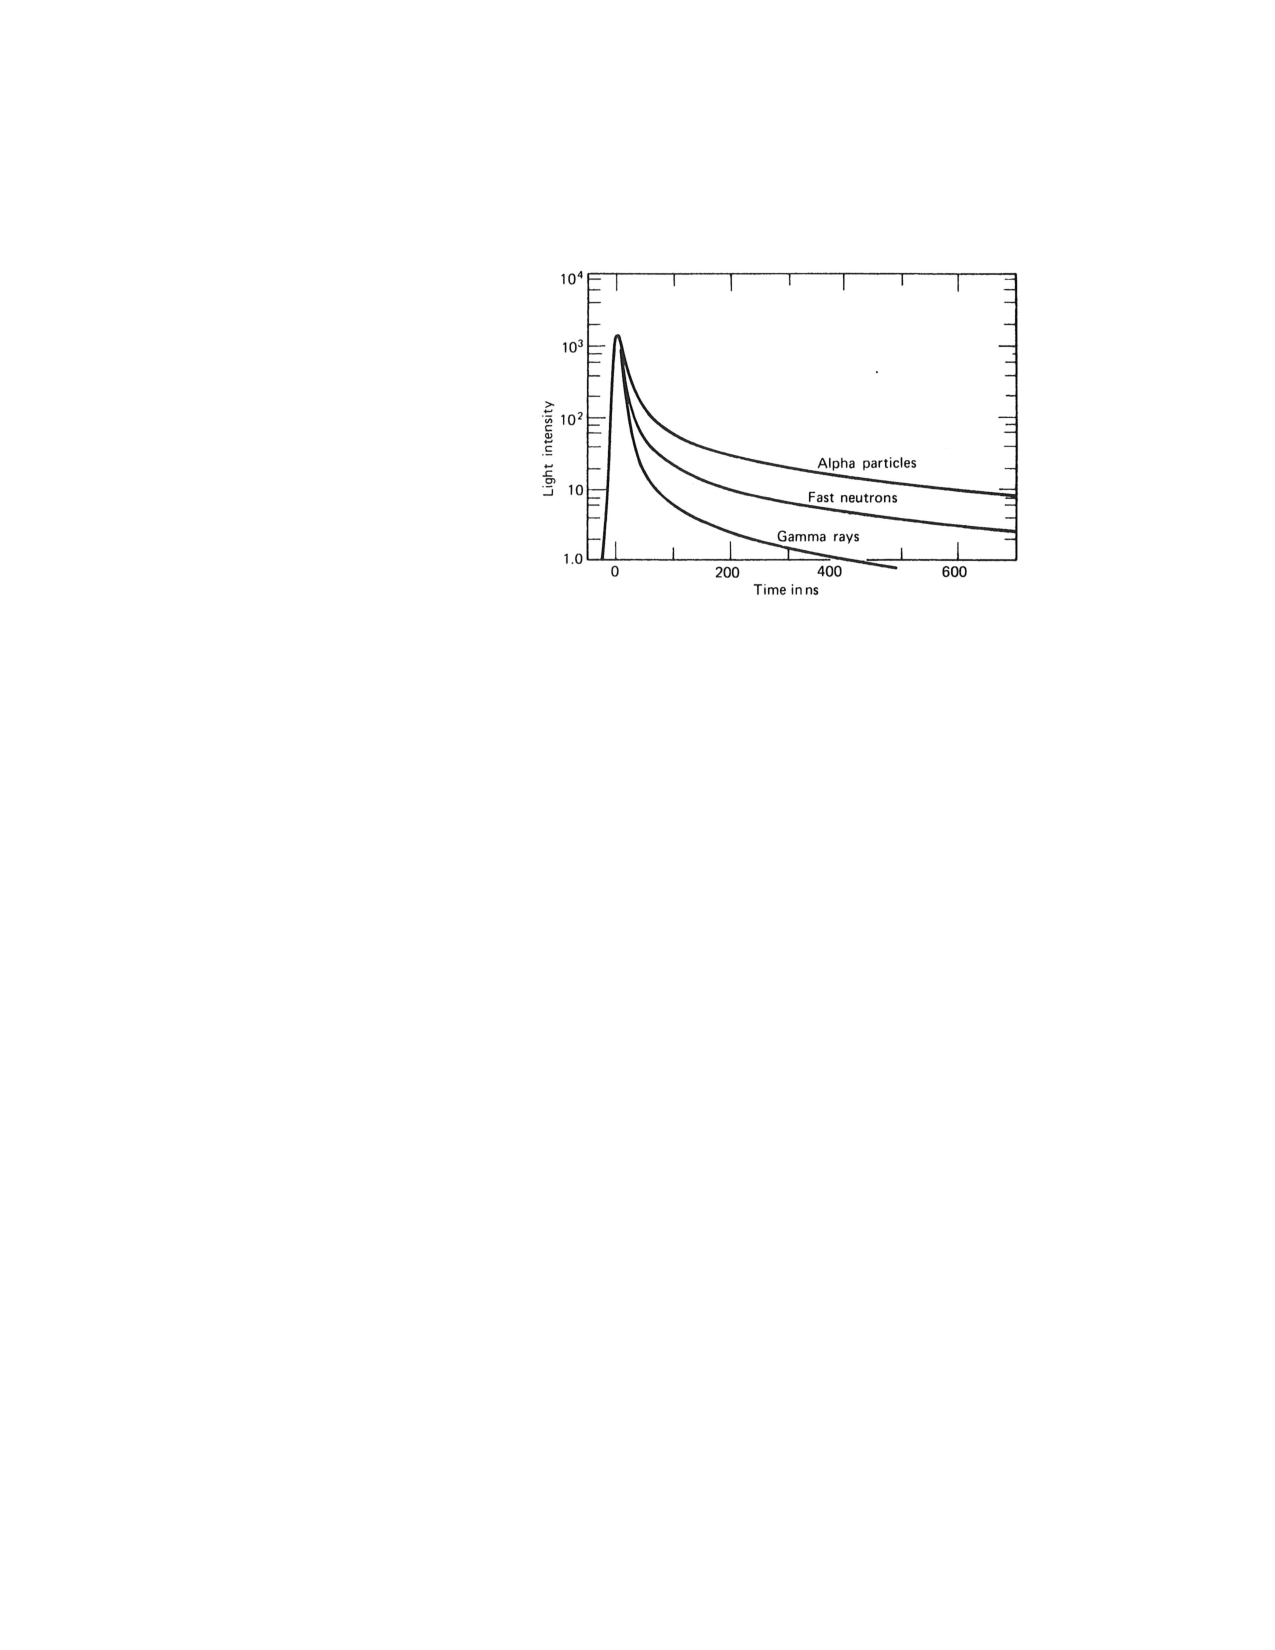
\includegraphics{Setup_Figs/pulse_shape.pdf}
    \caption{A cartoon illustration of pulse shape based on radiation type, in the same detecting material. The different types of radiation interact with the detecting material creating a fast and slow excitation. The ratio of these fast and slow excitations is based on the radiation, and expressed in the length of the decay tail. Picture taken from \citep{knoll00:rad_det_meas}.}
    \label{fig:pulse_discrimination}
\end{figure}

By plotting the pulse height against the decay tail time, neutrons and gammas can be separated. In this setup, this was done by sending the signal to a Mesytec MPD-4 (Multi-channel Pulse Discriminator) \citep{mesytec:_PSD}. This is a module built for pulse discrimination. It splits the signal, amplifies for the pulse height, and sends the other signal to a constant fraction discriminator (CFD), which outputs a timing signal that can be compared to a reference time from the RF beam pulsing. A CFD measures the time it takes for a pulse to decrease to a constant fraction of its original height. Both of these signals (the pulse amplitude and the TAC amplitude) are recorded in the data. Plotting these values in a two-dimensional plot distinguishes the gammas and neutrons, as in Figure \ref{fig:neutron}. There is a threshold cut off that removed most gammas from the spectrum.

\begin{figure}
    \centering
    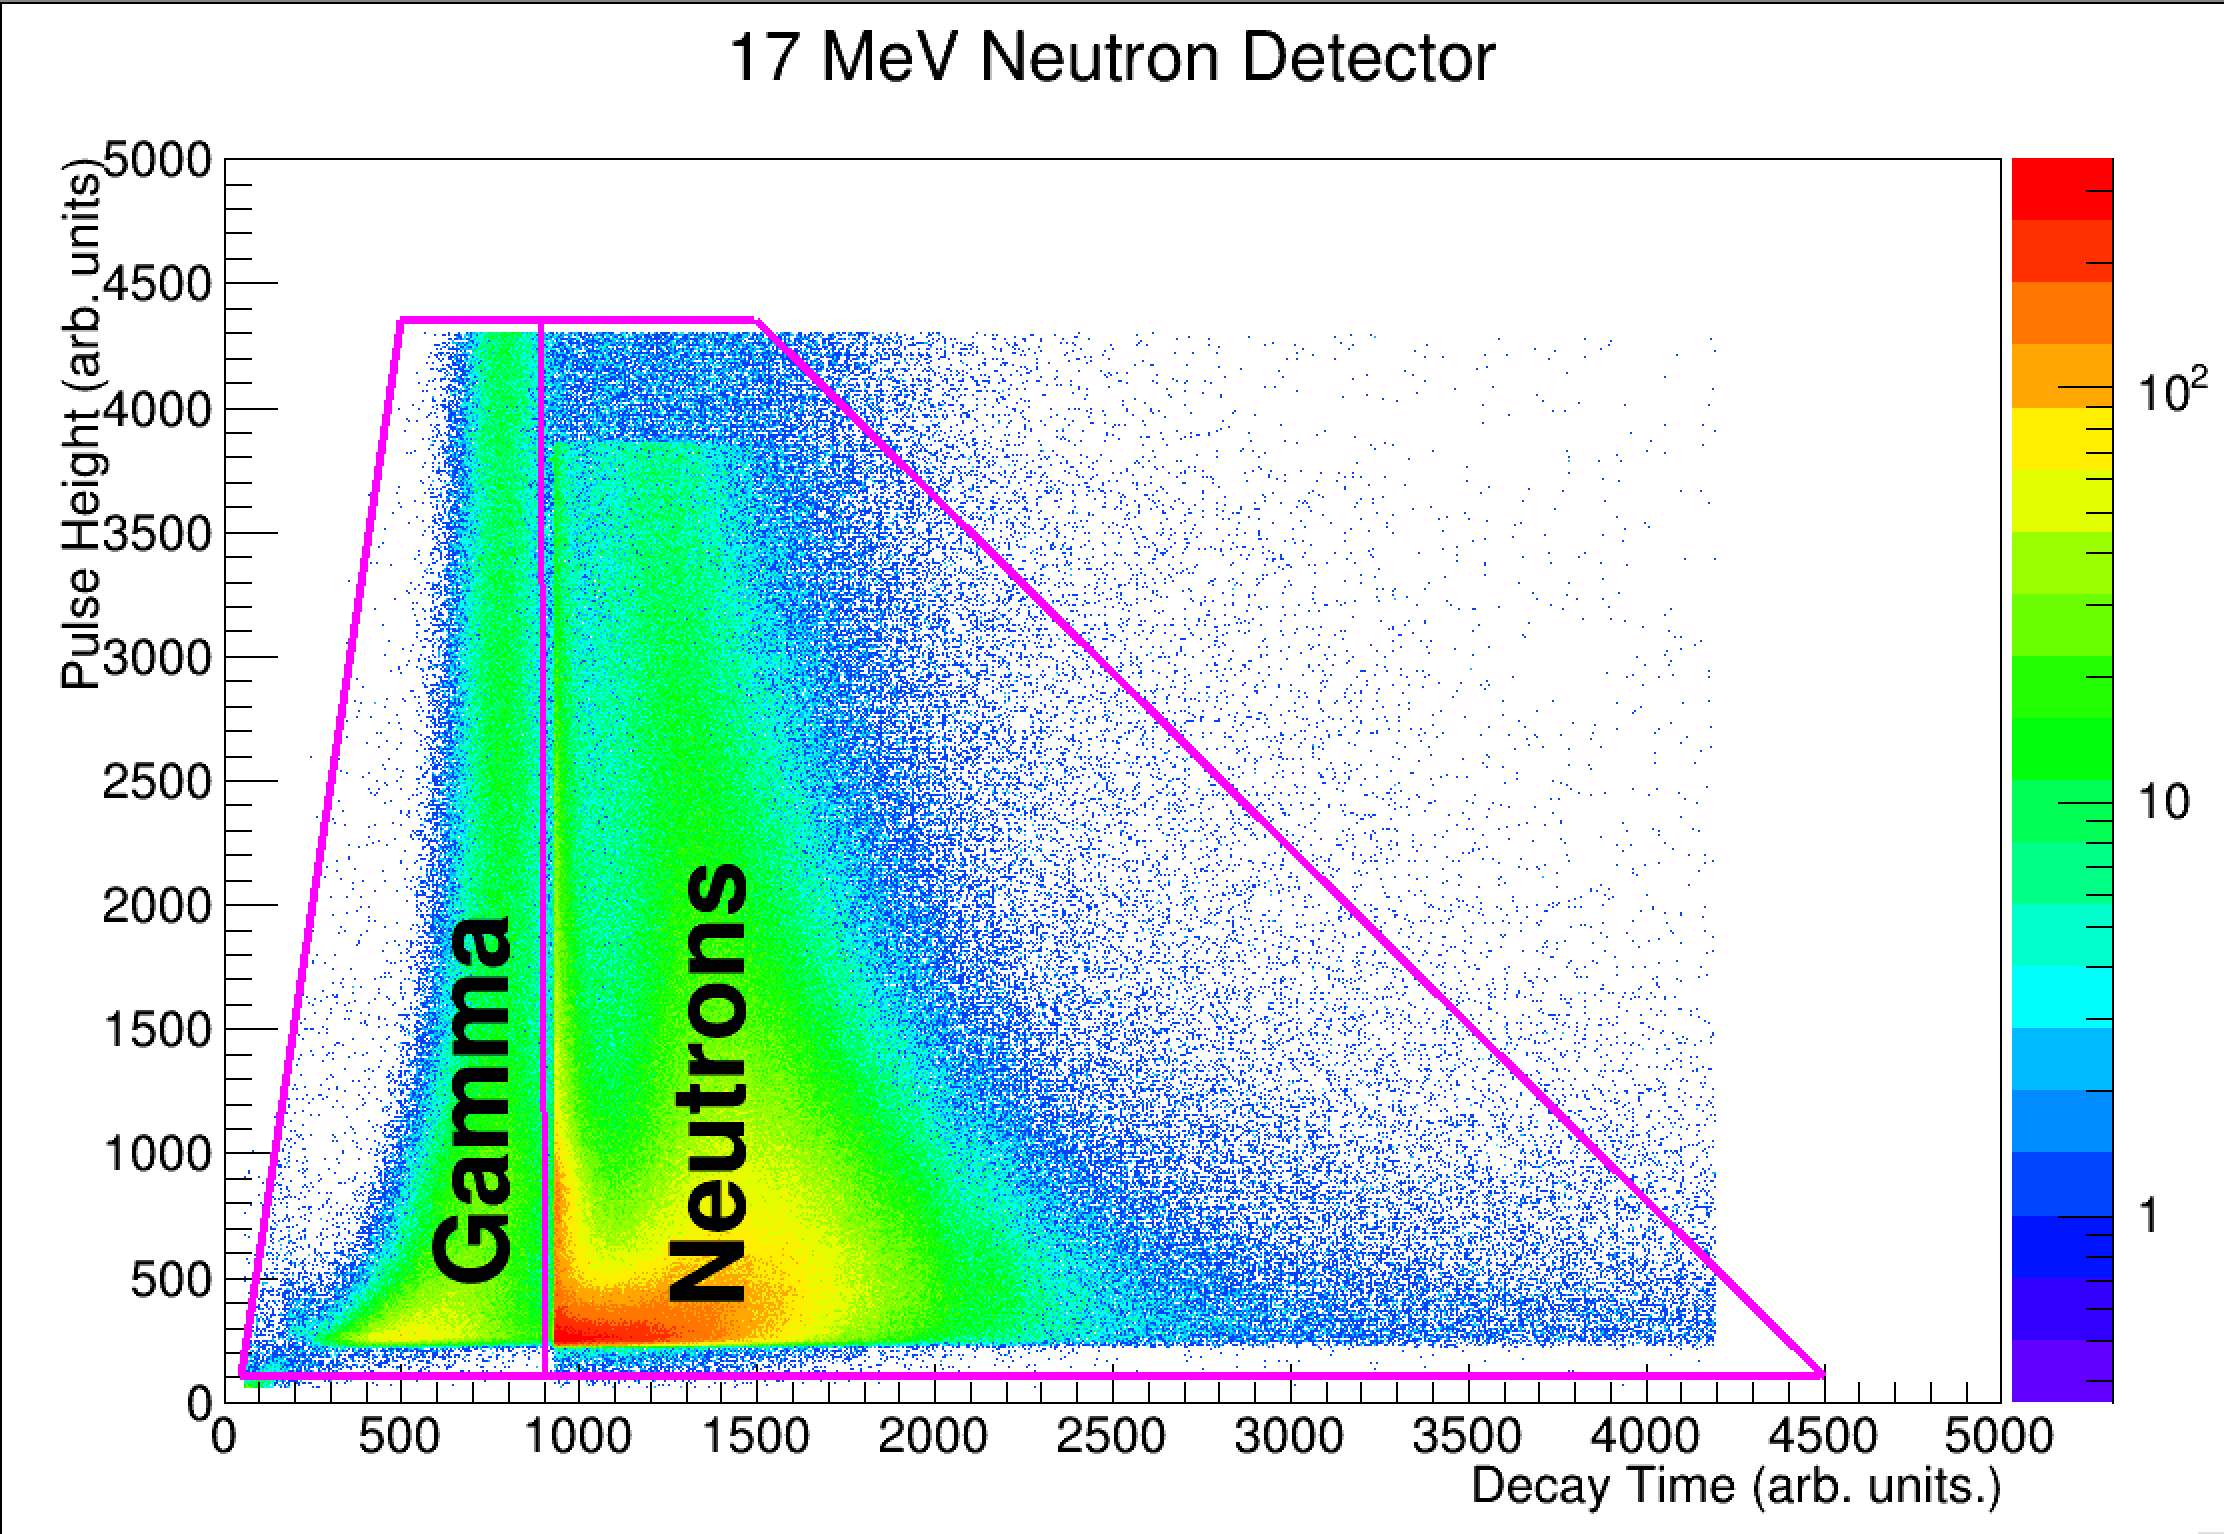
\includegraphics[scale=0.7]{Setup_Figs/17MeVNeutron.eps}
    \caption{Plot of the pulse height vs the decay time in the NE212 detectors. Two clear areas are seen. The leftmost, with the shorter decay time, is the gammas, while the more spread out peak on the right is neutrons.}
    \label{fig:neutron}
\end{figure}

Once the Si(Li) detectors were calibrated, each beam energy was run, with a total of four different targets across six energies. For each energy, the peaks in the electron spectra were identified with their respective isotopes, working under the assumption that only the lowest-lying states and the ground-state band would be populated significantly enough to see the electrons. These peaks are representative of the reaction cross section for that isotope. The K-electron of the $4^+\rightarrow2^+$ ground state transition for both nuclei of interest was clearly visible and clean at all energies, listed in Table \ref{tab:neutron_electron}. These K-electrons were used for the cross-section calculation.

\begin{table}[]
    \centering
    \caption{$4^+\rightarrow2^+ K-Electrons by Isotope$}
    \begin{tabular}{c|c}
    \toprule
         Isotope & Energy (keV)  \\
         \hline
         $^{154}$Gd & 197 \\
         $^{156}$Gd & 149 
         \bottomrule
    \end{tabular}
    \label{tab:neutron_electron}
\end{table}


To calculate the cross section, the formula
\begin{equation}
    \sigma=\frac{Yield}{\delta x*Q*\epsilon}\times \textit{Charge State} \times e
    \label{eq:xs}
\end{equation}
was used, where $\delta x$ is the target thickness, $Q$ is the integrated charge, \textit{Charge State} is the charge state of the incoming particles, $e$ is the electron charge, and $\epsilon$ is the efficiency of the Si(Li) detector at the electron energy. The $Yield$ is the area of the peak.

This then had to be compared with the neutron production cross section. Calculating the neutron flux was done using the formula
\begin{equation}
    \sigma_n = \frac{Neutrons}{\delta x*Q}
\end{equation}
where $\delta x$ and $Q$ are the same as used for the cross section and the efficiency of the neutron detectors is assumed to be \%100. This is not true in practice, and the neutron flux calculated are relative to each other. This area can be integrated over to get the number of neutrons seen during the run.

Table \ref{tab:neutrons} summarizes the results at each energy. Note, that the cross section is not reflective of the full cross section of the isotopes, but of the K-electrons for that transition. This ratio, of the cross-section to the neutron flux, was ultimately used to determine the running energy. The two higher energies, 20 and 21 MeV, have a ratio that agrees within error for both isotopes, indicating a plateau, in agreement with the expectation from Talys. Ultimately, 20 MeV was chosen for two reasons: to minimize any higher energy reaction channels, and because the neutron flux was lower in rate.

\begin{table}[]
    \centering
    \begin{tabular}{c|c|c|c|c|c}
        \toprule
        & \multicolumn{2}{c|}{Cross Section (mb)} & Neutron Flux & \multicolumn{2}{c}{Ratio ($\sigma/\Phi_n$)} \\
        Energy (MeV) & $^{154}$Gd & $^{154}$Gd & (neutrons/s) & $^{154}$Gd & $^{154}$Gd \\
        \hline
        16 & 0.126 (13) & 0.334 (25) & 1.247 (4) & 0.101 (10) & 0.268 (20)\\
        17 & 0.554 (54) & 1.273 (91) & 2.142 (13) & 0.259 (25) & 0.594 (43)\\
        18 & 3.124 (133) & 5.427 (233) & 4.281 (30) & 0.730 (31) & 1.268 (55)\\
        19 & 3.030 (172) & 5.327 (217) & 4.205 (25) & 0.721 (41) & 1.267 (52)\\
        20 & 5.618 (167) & 9.438 (275) & 5.806 (36) & 0.968 (29) & 1.626 (48)\\
        21 & 7.438 (267) & 12.827 (419) & 7.410 (54) & 1.004 (37) & 1.731 (58)\\ 
        \bottomrule
    \end{tabular}
    \caption{Summary of Energy Tests}
    \label{tab:neutrons}
\end{table}

\section{Electron Detection}

Silicon detectors are a commonly used particle detector, with good energy resolution. The detectors are semiconductors, using a $p-n$ junction to create a depletion region, which becomes the active detection region\citep{knoll00:rad_det_meas}. Semiconductors have a bandgap around 1eV. A cartoon of the bandgap can be seen in Figure \ref{fig:bandgap}. The $p-n$ junction takes two semi-conductor materials, one of $p$-type (an excess of holes in the valence band) and one of $n$-type (an excess of electrons in the conduction band) together. The holes and electrons mix, creating a depletion region, which becomes the active detection area. This region can be enlarged to some extent by putting a bias across the detector.

\begin{figure}
    \centering
    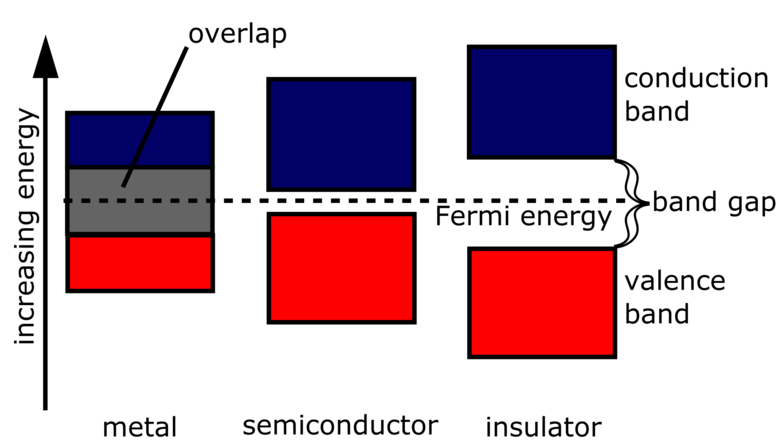
\includegraphics[scale=0.5]{Setup_Figs/semiconductor.png}
    \caption{Cartoon of how the bandgap works for insulators, conductors, and semiconductors. Insulators have a large band gap, conductors overlap, and semiconductors have a small bandgap.}
    \label{fig:bandgap}
\end{figure}

Because electrons are much more penetrating than protons or alphas of the same kinetic energy, it takes much more material to fully stop electrons. Silicon detectors only have active regions of 1mm-2mm thick, due to impurities, and cannot be made thick enough for the purposes of measuring electrons in the energy range of interest. Lithium-drifted silicon, colloquially Si(Li), detectors operate under the same principles as silicon detectors, but can be manufactured with larger depletion regions and a larger detectable energy range of electrons. These work by specifically introducing impurities, or doping, in this case lithium, to the detector, drifting it to create a $p-i-n$ junction. The $i$ region is also known as the intrinsic region, and is created by the drifting of the lithium, creating a highly purified region. The thickness of these detectors is only limited by the distance across which the lithium can be successfully drifted.

\subsection{Internal Conversion Electron Ball Spectrometer}
\label{sec:iceball}

The Internal Conversion Electron Ball Spectrometer (ICEBall) was developed at the University of Pittsburgh by Metlay et al. \citep{metlay92:_iceball_comm,metlay93:_iceball_comm}. Originally at the Spin Spectrometer at Oak Ridge National Laboratory, it was later stationed at the Wright Nuclear Structure Laboratory at Yale University with the YRAST Ball, until being brought to the University of Notre Dame and stationed in the Nuclear Science Laboratory West Target Room, on a dedicated beamline \citep{battaglia15:_iceball_176lu}.

Originally designed to go inside of large gamma detector arrays, ICEBall consists of six mini-orange spectrometers, cooled using liquid nitrogen for ideal energy resolution. The liquid nitrogen is administered using an autofill system with two thermal sensors for a start and stop signal. When the sensor closest to the detectors warms enough, liquid nitrogen is pumped into the system. A second sensor at the top of the dewar is used to stop the fill of liquid nitrogen before it overflows. This system fills in 15 to 20 minute intervals. ICEBall can be seen in Figure \ref{fig:open_iceball}, open for servicing.

\begin{figure}
    \centering
    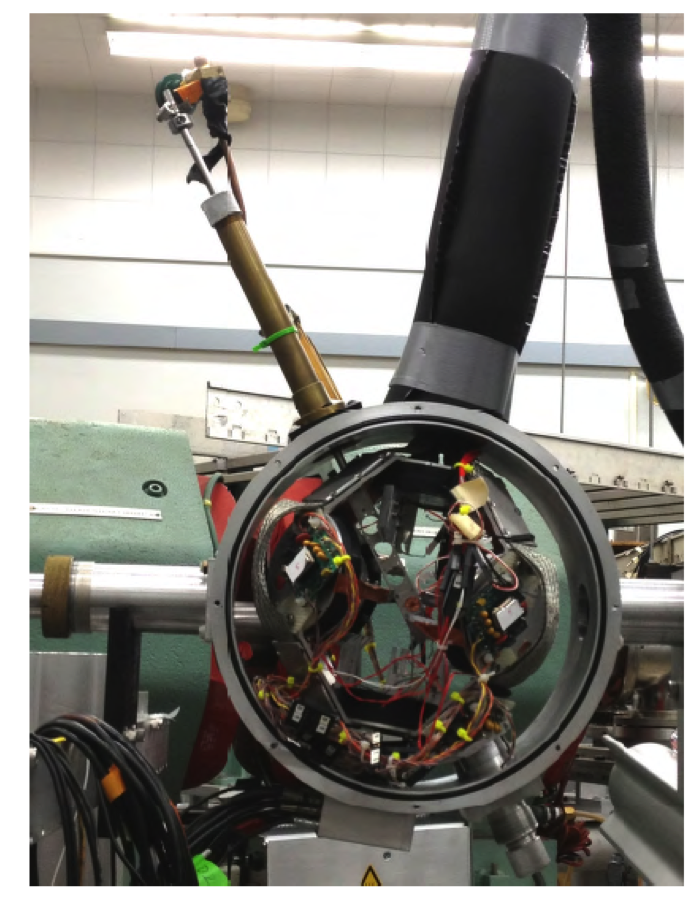
\includegraphics[scale=0.8]{Setup_Figs/Open_ICEBall.png}  
    \caption{Image of ICEBall, open for servicing. The beam would go from left to right in the picture. The target ladder is blank, in the center of ICEBall.}
    \label{fig:open_iceball}
\end{figure}

The Si(Li) detectors inside of ICEBall are 5 mm thick, with a surface area of 750 mm$^2$ \citep{metlay93:_iceball_comm}. Table \ref{tab:ICE_Det_Loc} summarizes the locations of the six Si(Li) detectors inside of ICEBall, using spherical coordinates. A thin aluminized mylar foil is placed in front of the Si(Li) detectors to block low-energy electrons and $\delta$-rays that successfully make it past the mini-orange filter (discussed in Section \ref{sec:mini_orange}).

\begin{table}[tpb]
    \centering
    \caption{ICEBall Detector Locations}
        \label{tab:ICE_Det_Loc}
    \begin{tabular}{c|c|c} \toprule
         Detector & $\theta$ & $\phi$  \\
         \hline
         1 & 90 & 79.2 \\ 
         2 & 270 & 100.8\\
         3 & 172 & 129.9\\
         4 & 198 & 31.7\\
         5 & 18 & 148.3\\
         6 & 355 & 50.1\\ \bottomrule
    \end{tabular}
    \\[2pt]
    \footnotesize
    The beam axis is the z-axis. $\theta$ is the angle in the xy-plane, where 0 degrees is beam left. $\phi$ is the azimuthal angle, with respect to the beam axis. All values are in degrees.
\end{table}

\subsubsection{Mini-Orange Spectrometer}
\label{sec:mini_orange}

Between the detectors and the target are mini-orange filters. First designed in the 1970s, mini-orange filters are a permanent magnet array surrounding a high-Z material, as seen in Figure \ref{fig:mini_orange} \citep{vanklinken72:mini_orange, vanklinken75:mini_orange}. In ICEBall, this material is tungsten, and the magnets are made of SmCo$_5$, and arranged in groups of 3. The tungsten acts as a blocker, lowering background from the target that can be due to $\gamma$ rays and heavy charged particles. The magnets create a field that bends electrons toward the detector, while bending positrons away from the detector, further lowering background noise. 

\begin{figure}
    \centering
    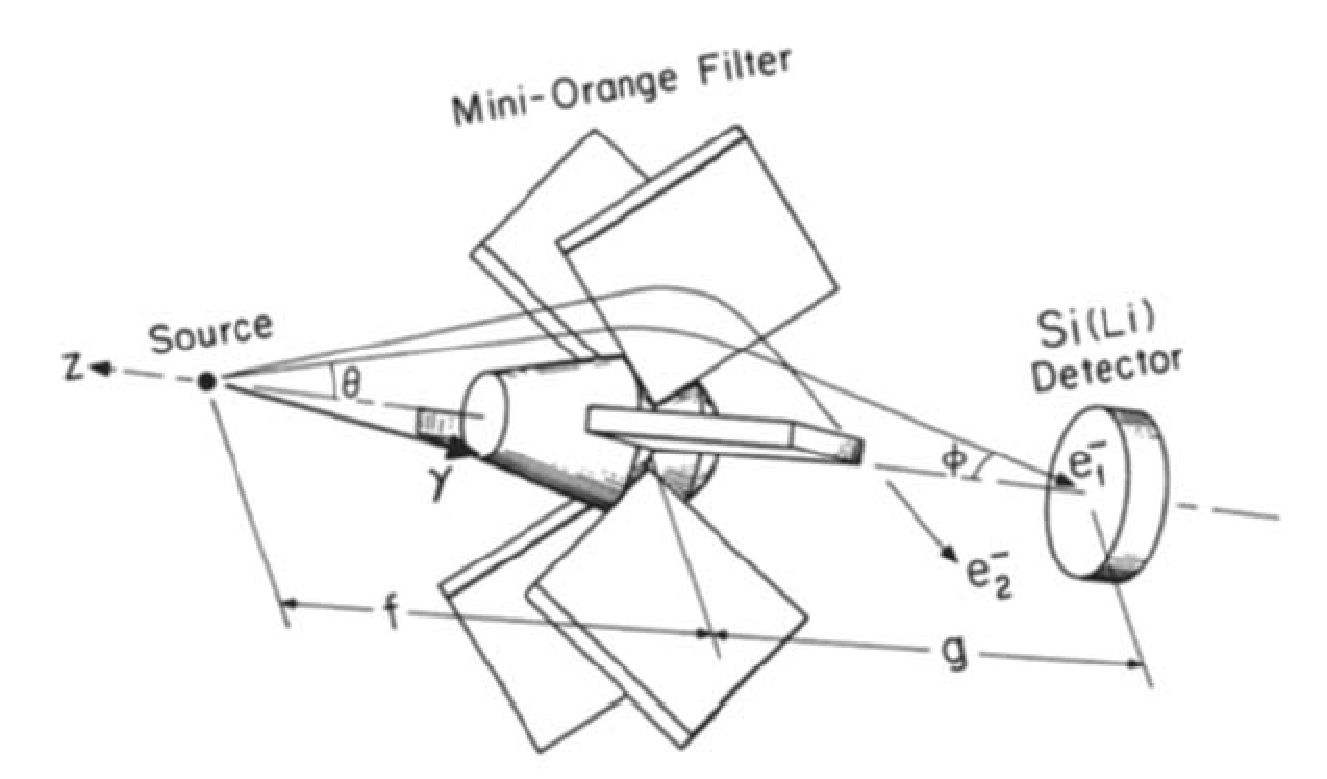
\includegraphics[scale=0.6]{Setup_Figs/mini-orange-metlay-figure.pdf}
    \caption{Graphic of the mini-orange filter. The central blocker keeps $\gamma$-rays from hitting the detector. The magnets bend electrons toward the detectors, and positrons away from the detectors. Being permanent magnets, they are optimized for a range of electron energies, and can cause overbending or underbending of electrons outside of that energy range, making the magnetic filter a factor in the efficiency. Taken from \citep{metlay93:_iceball_comm}}
    \label{fig:mini_orange}
\end{figure}

Compared to conventional spectrometers that sweep over electron energies by changing the magnetic field of the spectrometer, the mini-orange spectrometers are able to cover a wide range of energies at once. A drawback of this is the permanent magnets. The field is optimized for a range of energies, and must be pre-selected before the experiment. Switching magnets mid-experiment is not feasible, due to the downtime needed to warm-up the system, bring it to atmosphere, replace the filter, and then return the system to data taking conditions. Additionally, the efficiency of the system is a convolution of the detector's efficiency and the mini-orange filter in front of it, meaning each configuration must have a separate efficiency measurement. Tables \ref{tab:ICE_Magnet_G} and \ref{tab:ICE_Magnet_C} summarize the magnetic configurations of the mini-orange filters used in the experiments. The higher the magnetic strengths, the higher energy the peak efficiency of the mini-orange spectrometer, seen in Figure \ref{fig:filtercomp}. For the GEORGINA configuration, the magnetic strengths were all of similar values. For the Clovershare configuration, the filters were replaced on three detectors to enhance electron efficiency at higher energies.

\begin{figure}
    \centering
    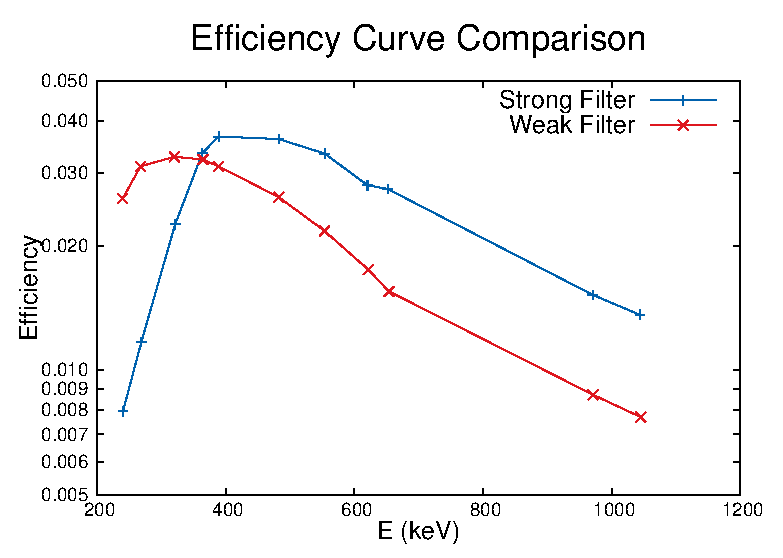
\includegraphics[scale=1]{Setup_Figs/FilterComparison.eps}
    \caption{An efficiency comparison of magnetic filters of two different strengths. The weak filter has been weakened by 70\% compared to the strong filter, using the Pitt split-pole spectrograph. Data from \citep{metlay92:_iceball_comm}.}
    \label{fig:filtercomp}
\end{figure}

\begin{table}[]
    \centering
    \caption{ICEBall magnetic strengths with GEORGINA}
     \label{tab:ICE_Magnet_G}
    \begin{tabular}{c|c|c} \toprule
         Detector & Filter & Strengths \\
         \hline
         1 & M13 & 815,740,830 \\ 
         2 & M15 & 939,911,949\\
         3 & M21 & 850,875,900 \\
         4 & M14 & 972,911,992\\
         5 & M18 & 856,913,963\\
         6 & M22 & 845,900,900\\ \bottomrule
    \end{tabular}
    \\[2]
    \footnotesize
    Magnetic strengths of the mini-orange filters used in the GEORGINA experiments, listed in Gauss. All the magnetic strengths are similar and geared for efficiency peaking at approximately 300-400 keV.
\end{table}

\begin{table}[]
    \centering
    \caption{ICEBall magnetic strengths with Clovershare}
     \label{tab:ICE_Magnet_C}
    \begin{tabular}{c|c|c} \toprule
         Detector & Filter & Strengths \\
         \hline
         1 & M13 & 815,740,830 \\ 
         2 & M20 & 1228,1292,1265\\
         3 & M21 & 850,875,900 \\
         4 & M2 & 1411,1420,1410\\
         5 & M16 & 1286,1340,1285\\
         6 & M22 & 845,900,900\\ \bottomrule
    \end{tabular}
    \\[2]
    \footnotesize
    Magnetic strengths of the mini-orange filters used in the Clovershare experiments, listed in Gauss. The magnetic strengths are mid-energy range and high-energy range for efficiency.
\end{table}

\subsection{Calibration}

ICEBall is energy and efficiency calibrated using two sources: $^{133}$Ba and $^{207}$Bi. The specific properties of the two sources are listed in Table \ref{tab:ICE_Cal_Source}. The $^{207}$Bi covers the high-energy regime, with lines around 500 keV and 1000 keV. The $^{133}$Ba covered energies from 200 to 400 keV. Both sources are low activity, preventing incomplete or overlapping charge collection from hindering the resolution of the detectors during calibration runs. 

\begin{table}[]
    \centering
    \caption{ICEBall calibration sources}
        \label{tab:ICE_Cal_Source}
    \begin{tabular}{c|c|c|c|c} \toprule
         Source & Date Measured & Activity & Energy (keV) & Intensity (\%)\\
          \hline 
         $^{133}$Ba & May-4-2012 & 0.331(7) $\mu$Ci & 240.413 & 0.331 \\
         & & & 266.868 & 0.698 \\
         & & & 320.032 & 1.308 \\
         & & & 347.866 & 0.370 \\
         \hline
         $^{207}$Bi & May-4-2012 & 0.306(8) $\mu$Ci & 481.697 & 1.562 \\ 
         & & & 554.4 & 0.469 \\
         & & & 975.657 & 7.243 \\
         & & & 1048.1 & 1.838 \\\bottomrule
    \end{tabular}
    \\[2]
    \footnotesize
    Calibration source information for ICEBall. The energies and the respective intensities are listed for each source. Intensities are taken from \cite{trzaska90:_calibration}. The intensity of the 347 keV line in $^{133}$Ba is both the 384K and 356L intensities combined.
\end{table}

The energy calibration is assumed to be quadratic in nature, although both linear and quadratic calibrations are performed. Figure \ref{fig:iceball_cal} shows both of these fits and their respective residuals for one of the Si(Li) detectors. These values are summarized in the next chapter for each experiment.

\begin{figure}
    \centering
    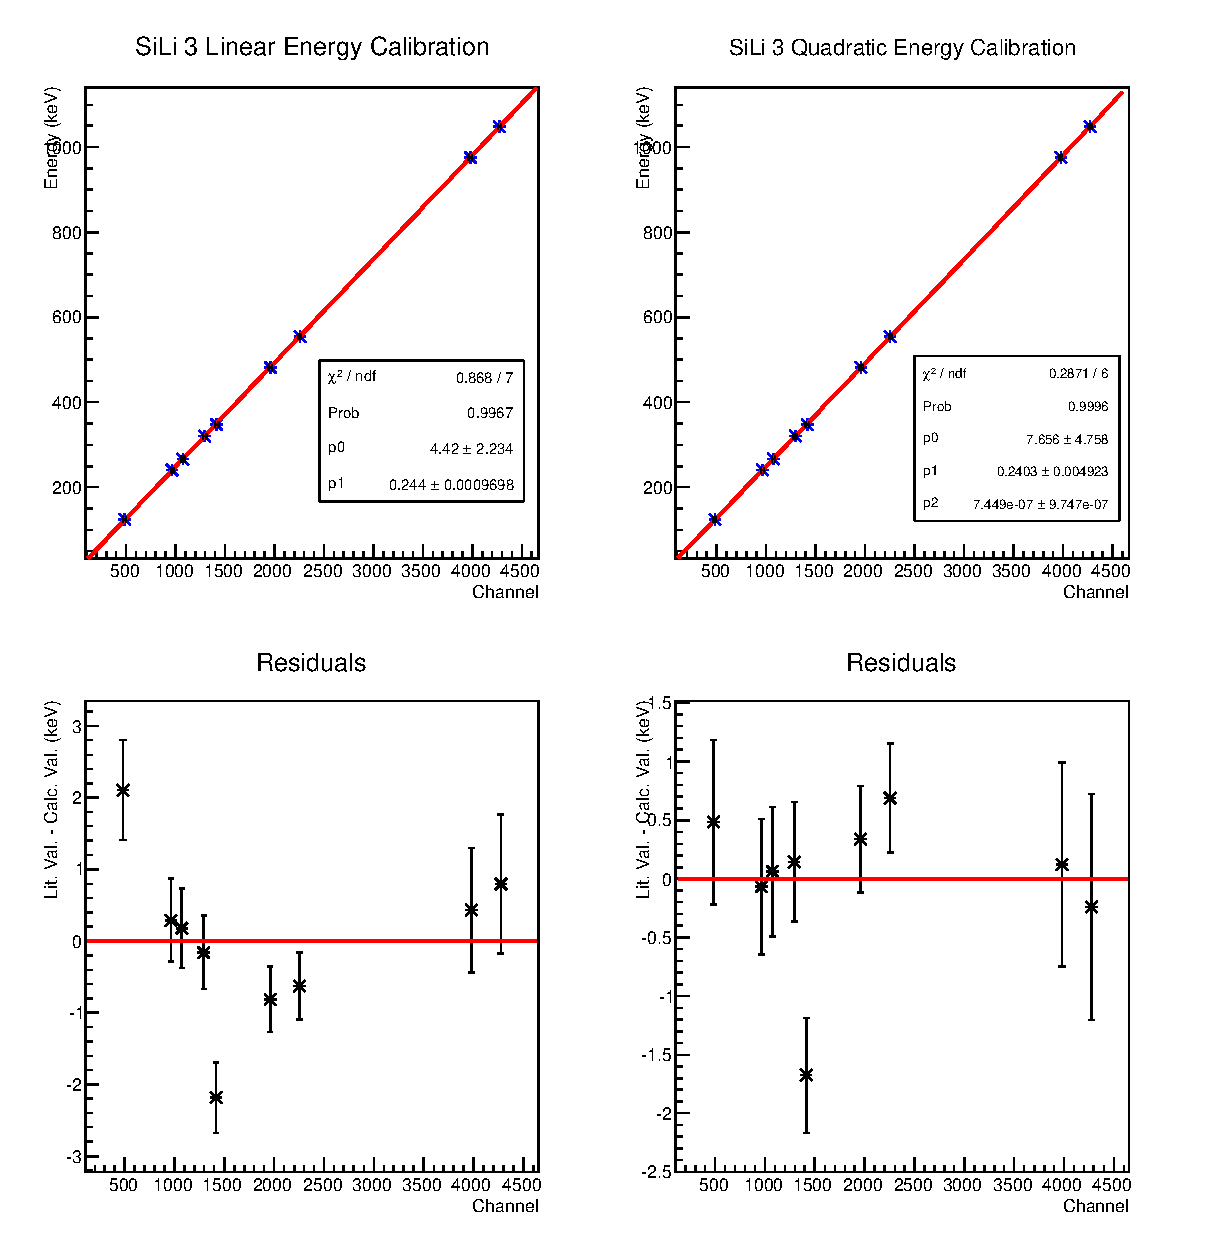
\includegraphics[scale=0.75]{Setup_Figs/sili_3.eps}
    \caption{Linear and quadratic energy calibrations of one Si(Li) detector, using the electron energies listed in Table \ref{tab:ICE_Cal_Source}. The top graphs show the calibrations, while the graphs beneath show the respective residuals. The calibration is in much better agreement in the quadratic fit, as seen in the residuals.}
    \label{fig:iceball_cal}
\end{figure}

The efficiency calibration is fitted to equation
\begin{equation}
    ln(\epsilon) = p_1+p_2ln(E)+p_3E.
    \label{eq:SiLi_Eff}
\end{equation}
The efficiency is a convolution of the magnetic configuration and the inherent detector efficiency. Using the efficiency points, the analytic expression for the efficiency was determined empirically in previous work \citep{battaglia15:_iceball_176lu}. These experimental values are summarized in the next chapter for each experiment.

\section{Gamma Detection}

Gamma radiation is highly penetrating, making semiconductor detectors of normal purity unusable, as they have limitations on the depth of the depletion region that are nowhere near the necessary depths needed for fully stopping gamma radiation. The depletion depth is inversely proportional to the number of impurities in the material \citep{knoll00:rad_det_meas}. High-purity germanium, also known as intrinsic germanium, detectors decrease these impurities to increase the depletion depth, resulting in depths of several centimeters.

Like other semi-conductor detectors, there are dead layers that attenuate the radiation. Generally, this attenuation is negligible above 200 keV. These detectors have a high resolution due to the small bandgap of 0.7 eV in germanium. This small bandgap comes at a price, and HPGe detectors can only be operated at liquid nitrogen temperatures, as putting any voltage on a room temperature HPGe would result in high leakage currents and noise, making detection impossible.

\subsection{GEORGINA}

The GErmanium detector Online aRray for Gamma ray spectroscopy in Nuclear Astrophysics (GEORGINA) is a compact array of high-purity germanium (HPGe) detectors for $\gamma$-ray experiments\citep{isnap18:_georgina}. The detectors are 100\% relative efficiency (as compared with a $3"\times3"$ NaI detector at 1332 keV). These detectors were designed for use with low cross-section astrophysical capture reactions, meant to cover a large solid angle. The array has a total of five detectors, two of which were used in this experiment. The detectors were designed with the crystal at a $90^{\circ}$ from the cold-finger, as seen in Figure \ref{fig:georgina}.

\begin{figure}
    \centering
    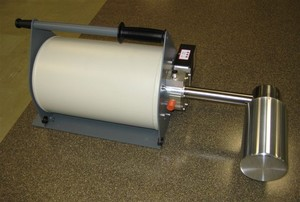
\includegraphics{Setup_Figs/georgina_example.png}
    \caption{An example of one of the GEORGINA detectors. The crystal is at a $90^{\circ}$ from the cold finger, allowing the long side of the crystal to be placed next to the target, to optimize solid angle coverage. In the experiment, the circular face of the crystal was placed toward the target.}
    \label{fig:georgina}
\end{figure}

One of the two detectors had Bismuth Germanate (BGO) detectors from Argonne National Laboratory around it to cut down on background from incomplete charge collection. BGO detectors have a high efficiency, but poor resolution, and are good to use as a veto system. In the event that a gamma-ray does not deposit its full energy in the HPGe crystal, the BGO detectors surrounding the crystal should pick up the remaining energy. This indicates the event was incomplete in energy and should be excluded from the data. This is a manual cut made during the analysis procedure by looking at the data from the BGO detectors.

\subsection{CloverShare}

CloverShare is a group of nine HPGe clover detectors with BGO shields, that originated at Yale University as part of the YRAST Ball array \citep{beausang00:_yrast}. They were sent to various laboratories and universities for series of experiments, including the NSL. Two campaigns of experiments were run with CloverShare, each one involving an ICEBall experiment.

The CloverShare detectors are large, segmented HPGe detectors, with fitted BGO shields, seen in Figure \ref{fig:clover_example}. Each detector is segmented into four crystals, resembling a clover. Due to the "add-back" capability of these detectors, summing over the close-proximity crystals, the detectors each have a total relative efficiency \~150\%, whereas each individual crystal is approximately 20\% efficient. In the first of the two experiments, 7 detectors were used. In the second, 5 were used, as two experienced pre-amplifier problems during the previous campaign. The detectors used biases between -3000 and -4000 V, and were kept cold using a liquid nitrogen autofill system.

\begin{figure}
    \centering
    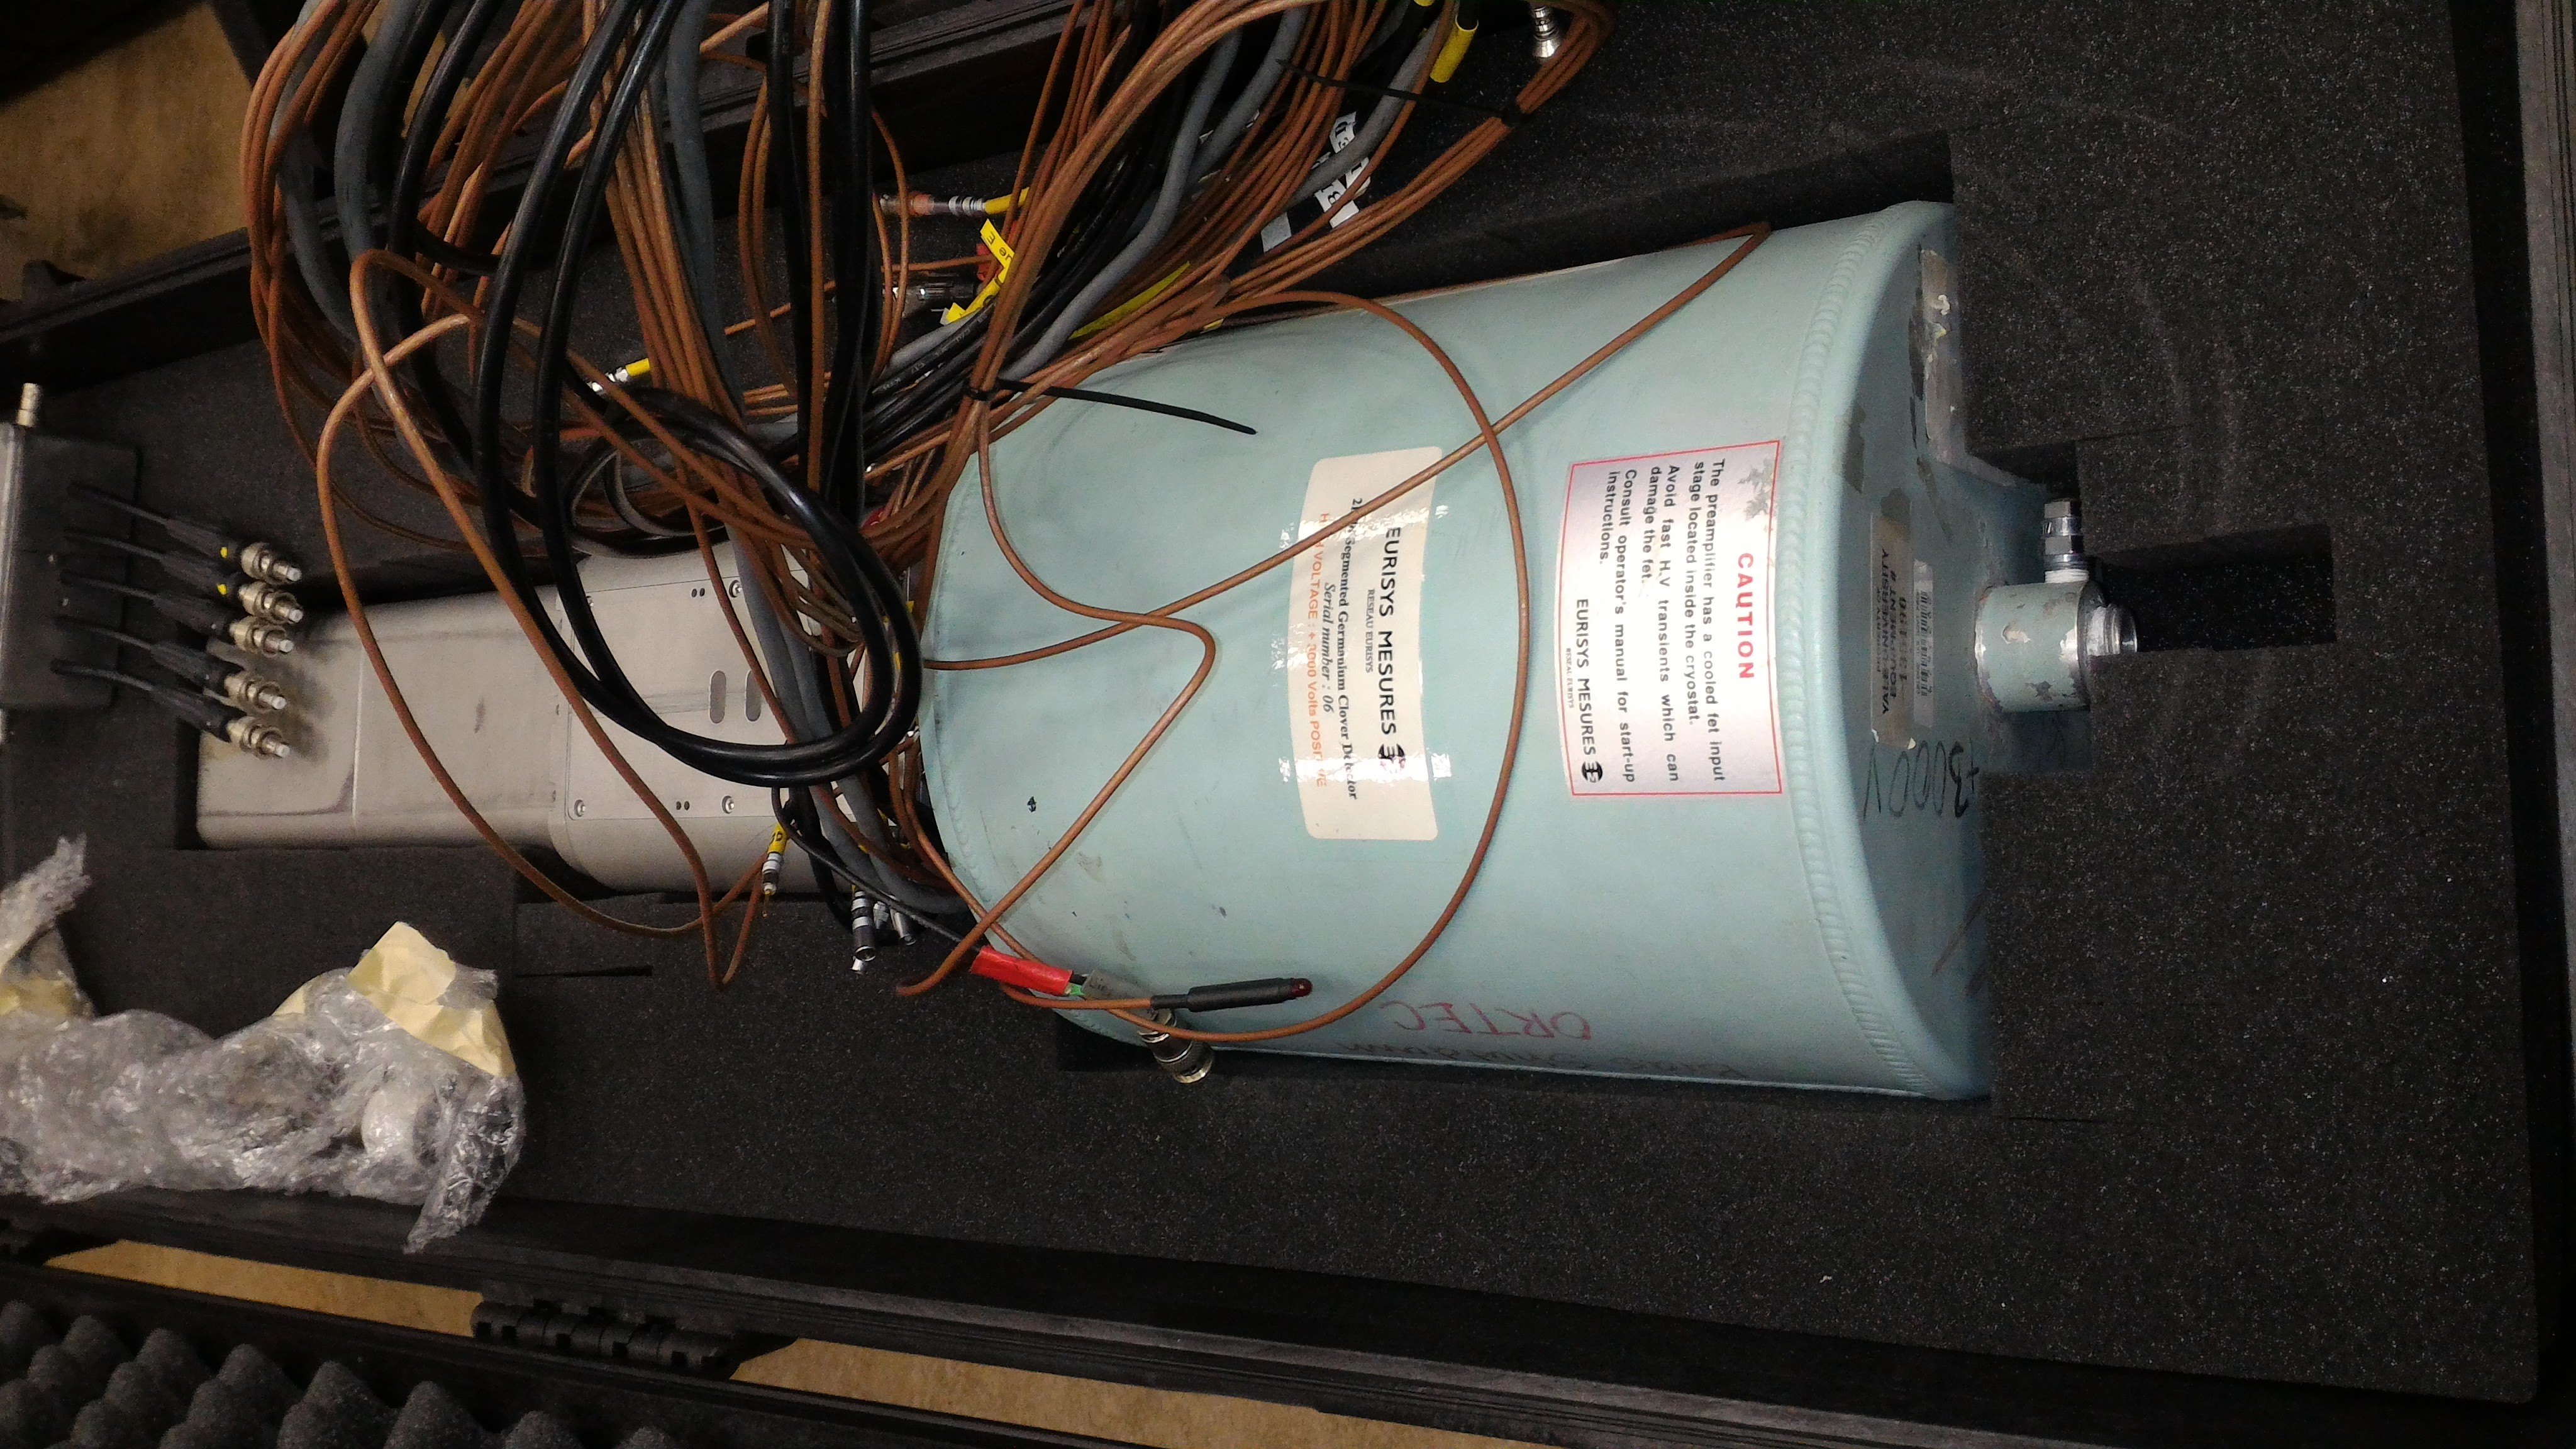
\includegraphics[scale=0.1]{Setup_Figs/P_20160118_094821.jpg}
    \caption{Example of one of the Clovershare detectors.}
    \label{fig:clover_example}
\end{figure}

\subsection{Calibration}
\label{sec:clover_cal}

Both sets of detectors were calibrated using a $^{152}$Eu source, in addition to the ICEBall sources. The information about the sources is in Table \ref{tab:GEORGINA_Cal_Source}. The $^{152}$Eu source was not designed to sit perfectly on the target ladder, while the two ICEBall sources were. So, even though the Eu source was attached to the target ladder for the GEORGINA calibration, using it as a measure of absolute efficiency was not possible. For the CloverShare calibration, the $^{152}$Eu source was placed on the individual detectors instead of centered in ICEBall. To use the $^{152}$Eu for the efficiency, a linear extrapolation of the efficiency of the 344 keV line was done using the 303 keV and 356 keV lines in $^{133}$Ba. All points in the Eu were then scaled based on this. Additionally, several background lines could be used to extend the energy calibration up to 2700 keV. The energy calibration was fit to a polynomial, and fits up to the fifth order were done to find the best calibration without overfitting. For examples of these fits, see the next chapter. All points in the Eu were then scaled based on this. A characteristic fit of the efficiency of these detectors can be seen in Figure \ref{fig:clover_eff}.

\begin{table}[]
    \centering
    \small
    \caption{GEORGINA calibration sources}
    \begin{tabular}{c|c|c|c|c} \toprule
         Source & Date Measured & Activity & Energy (keV) & Intensity (\%)\\
          \hline 
         $^{133}$Ba & May-4-2012 & 0.331(7) $\mu$Ci & 80.997 & 0.3406 \\
         & & & 276.398 & 7.164 \\
         & & & 302.853 & 18.33 \\
         & & & 356.017 & 62.05 \\
         & & & 383.851 & 8.94 \\
         \hline
         $^{207}$Bi & May-4-2012 & 0.306(8) $\mu$Ci & 569.702 & 97.75 \\ 
         & & & 1063.662 & 74.09 \\
         \hline
         $^{152}$Eu & & & 121.7825 & 28.65 \\
         & & & 244.6989 & 7.582 \\
         & & & 344.281 & 26.6 \\
         & & & 411.115 & 2.262 \\
         & & & 443.965 & 3.125 \\
         & & & 778.903 & 13.017 \\
         & & & 867.39 & 4.26 \\
         & & & 964.055 & 14.758 \\
         & & & 1085.842 & 10.062 \\
         & & & 1089.7 & 1.738 \\
         & & & 1112.087 & 13.587 \\
         & & & 1408.022 & 20.945 \\\bottomrule
    \end{tabular}
    \footnotesize
    \item Calibration source information for GEORGINA. The energies and the respective intensities are listed for each source. Intensities are taken from \cite{trzaska90:_calibration}. The  $^{152}$Eu does not have activity and intensity, as it was normalized to the $^{133}$Ba.
    \label{tab:GEORGINA_Cal_Source}
\end{table}

The efficiency calibration is fitted to equation
\begin{equation}
    ln(\epsilon) = a_0-(a_1+a_2\times e^{-a_3\times E})\times E^{-a_4\times E}\times ln(E).
    \label{eq:Ge_Eff}
\end{equation}
A characteristic fit can be seen in Figure \ref{fig:clover_eff}. The CloverShare detectors were also calibrated using a $^{56}$Co source that was created on the FN accelerator days before the experiment. The information about the source is in Table \ref{tab:Co_Energy}. 

\begin{table}[t]
    \centering
    \caption{$^{56}$Co Calibration Information}
    \label{tab:Co_Energy}
    \begin{threeparttable}
    \begin{tabular}{c|c}
    \toprule
         Activity & $\gamma$ Energy (keV)  \\ \hline
         6.44 $\mu$Ci\tnote{a} & 846.77 \\
         & 977.372 \\
         & 1037.843 \\
         & 1175.101 \\
         & 1238.288 \\
         & 1360.212 \\
         & 1771.357 \\
         & 2015.215 \\
         & 2034.791 \\
         & 2598.5 \\
         \bottomrule
    \end{tabular}
    \begin{tablenotes}[para]
    Energies used in $^{56}$Co for calibration, as well as activity.
    \newline\item[a] Measured on Mar-16-2016
    \end{tablenotes} 
\end{threeparttable}
\end{table}

\begin{figure}[t]
    \centering
    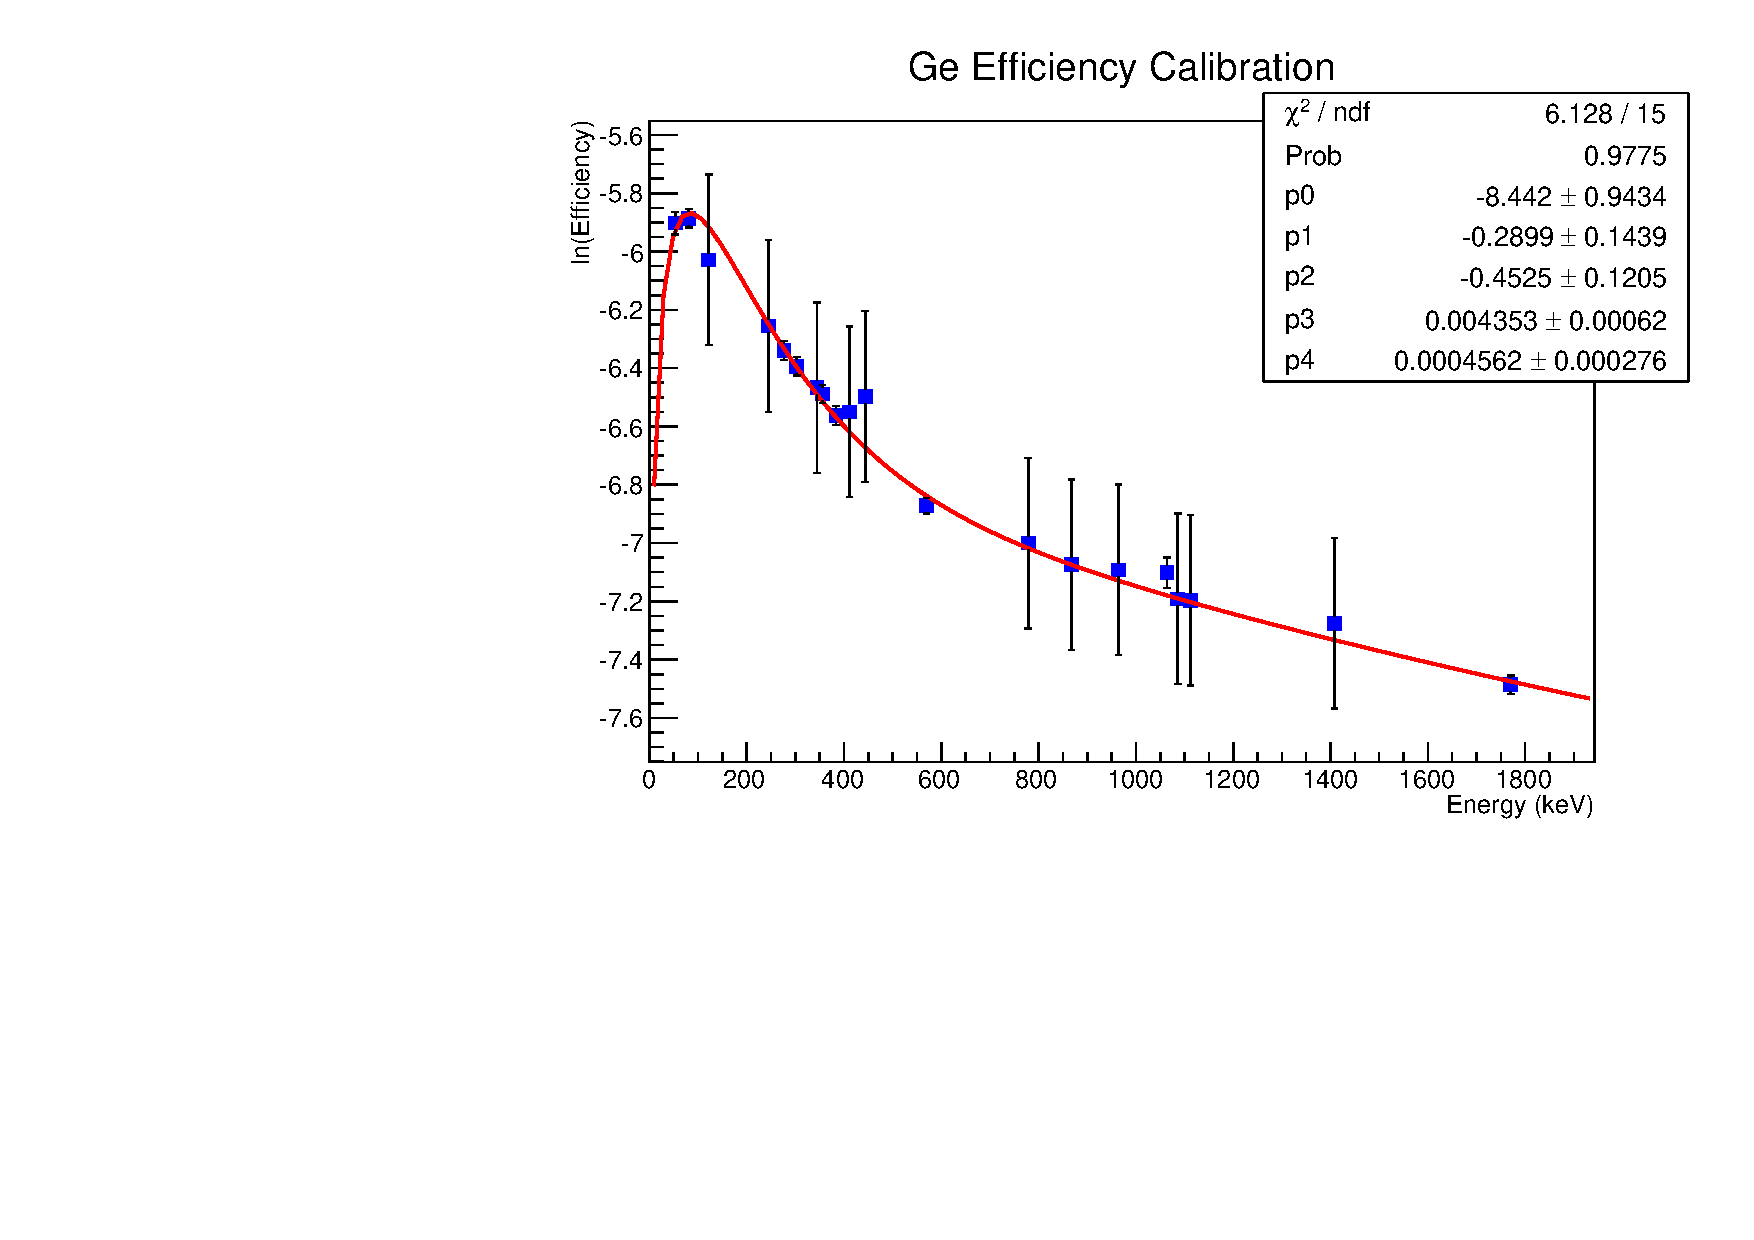
\includegraphics[scale=0.7]{Setup_Figs/Clover1_Eff_05232017.pdf}
    \caption{A characteristic fit of the Clovershare detector efficiencies. The points with large error bars are the $^{152}$Eu points, as the scaling of the points caused a large uncertainty, compared to the $^{207}$Bi and $^{133}$Ba.}
    \label{fig:clover_eff}
\end{figure}

As the clovers are comprised of four separate crystals, the efficiency was taken for the individual leaves, and once the detectors had been calibrated, they were summed together. Figure \ref{fig:Clover_ind_vs_sum} shows the comparison. As is expected, there is a small improvement in the higher energies. This is due to the summation of otherwise incomplete charge collection due to compton scattering within individual crystals. This did cause the efficiency at lower energies to appear lower, but this is due to the summing of cascades of energies over the segments. The summed crystals were used for analysis, and will be used in spectra from here on forward.

\begin{figure}[hbt!]
    \centering
    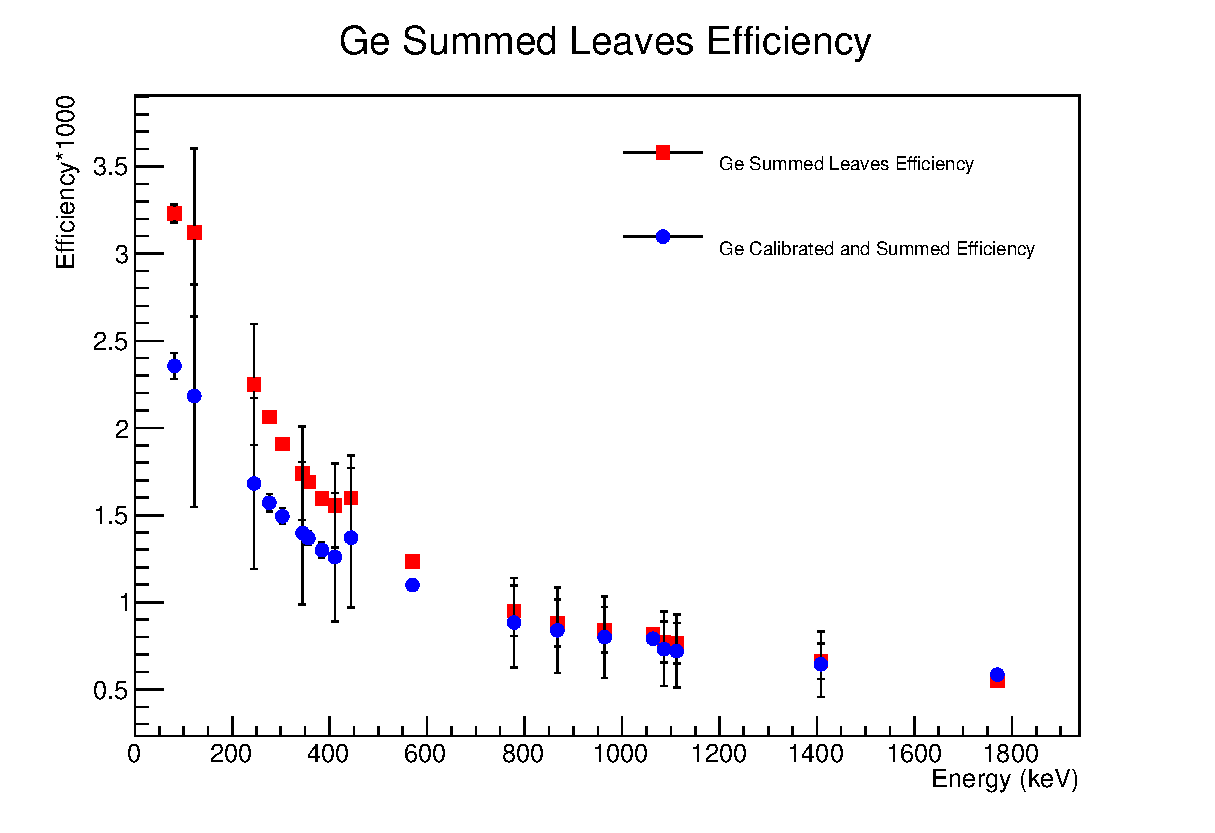
\includegraphics[scale=0.7]{Setup_Figs/Efficiency_ind_vs_sum.eps}
    \caption{Efficiency of a CloverShare detector, with the individual leaves' efficiency summed together, compared to the efficiency of the leaves calibrated and summed together. The different colors/shapes indicate the different sources, as labeled.}
    \label{fig:Clover_ind_vs_sum}
\end{figure}

Each leaf of the clovers was energy calibrated. An unusual trend in the residuals was found in all cases, as seen in Figure \ref{fig:Clover_ene_res}. This trend could not be corrected for by using a higher-order polynomial, as is usually the case for integral non-linearities in multi-channel analyzers \citep{knoll00:rad_det_meas}. Instead, this appears to be a differential non-linearity in the electronics, resulting in discontinuities. The electronics used for the experiment are not primarily used with detectors of this sensitivity.

\begin{figure}
    \centering
    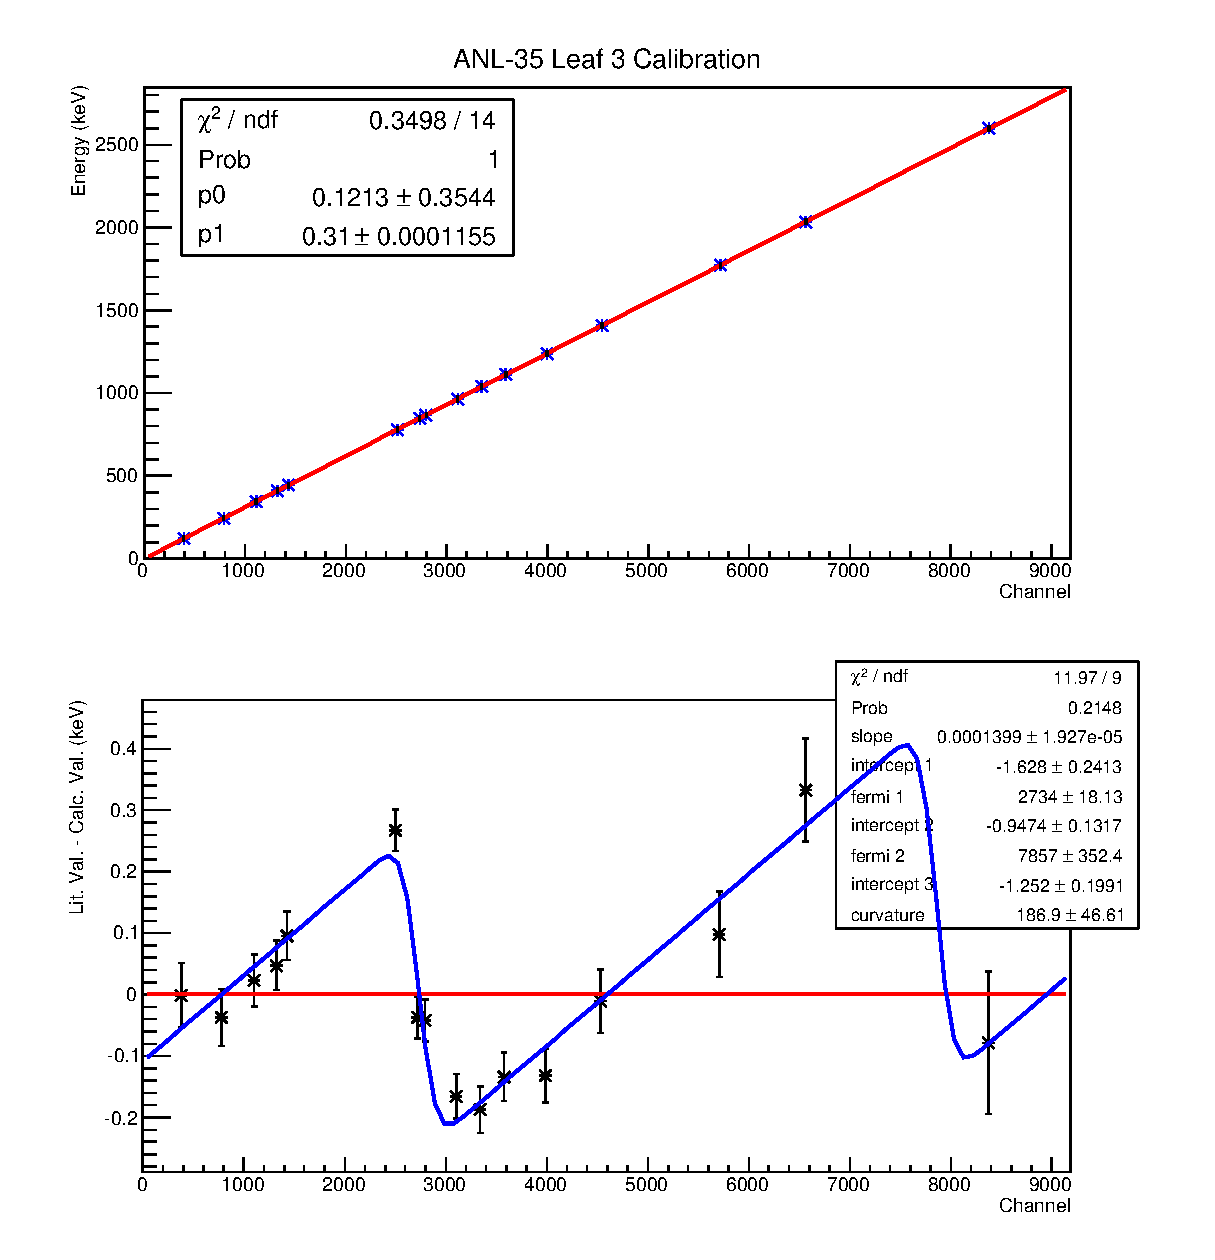
\includegraphics[scale=0.7]{Setup_Figs/Clover_res_cal.eps}
    \caption{A look at the energy calibration of an individual leaf in an HPGe Clover detector. The upper graph is a linear calibration. The lower graph is a look at the residuals. For HPGe detectors, $\pm0.4$ keV is not a good energy calibration. Here, the sawtooth fit that was derived from the differential non-linearity in the electronics is seen fitted to the data.}
    \label{fig:Clover_ene_res}
\end{figure}

\section{Target Fabrication}

Electrons must escape the target for detection. All materials have some stopping power for radiation, based on the material, thickness, and type of particle. The Beta-Bloch formula can be used to calculate this stopping power, with several programs, including SRIM, created to make and tabulate these values\citep{ziegler10:_srim}. A thicker target causes energy loss and straggling effects, blurring out the conversion electron spectrum, meaning a thinner target is a more ideal situation.

Enriched, self-supporting Samarium targets were used for this experiment. Table \ref{tab:target} has the enrichment and thickness of the targets used. The material started as Sm$_2$O$_3$. Using the reaction
\begin{equation}
    Sm_2O_3 + Hf \xrightarrow{} HfO_2 + Sm
    \label{eq:sm_hf}
\end{equation}
at a temperature of 1520-1820 K the Samarium was extracted as a metal and Halfnium was used as a reductant\citep{clifford02:_target}. Once cooled, it was rolled as thin as possible. Samarium easily oxidizes, stagnating the rolling process, as too much work on the material at once could cause instantaneous oxidization, resulting in the loss of the target. Rolling had to be done incrementally to prevent overheating the material and causing instantaneous oxidization.

\begin{table}[]
    \centering
    \caption{Target Enrichment and Thickness}
    \begin{tabular}{c|c|c}
    \toprule
         Isotope & Enrichment (\%) & Thickness (mg/cm$^2$) \\
         \hline
         $^{152}$Sm & $>98$ & 1.44  \\ 
         $^{154}$Sm & $>98$ & 1.7 \\ 
         \bottomrule
    \end{tabular}
    \label{tab:target}
\end{table}

\section{Experimental Configuration and Operation}

\subsection{Experimental Beam Operation}

The experiments with GEORGINA were done using a bunched beam, creating a timing reference to help identify events of interest. The beam was bunched before the accelerator, with a time separation of 600 ns between bunches and a full-width half-maximum of 16 ns for the bunch. The use of this timing reference is shown in Figure \ref{fig:bunched}. Clear separation of the bunches is visible. The accelerator was run with a terminal voltage of 6.64 MV, with $^{4}$He$^{2+}$ being sent through the machine, resulting in a beam of energy 20 MeV, including the initial 60 kV kick from the HIS. 

\begin{figure}
    \centering
    \includegraphics[scale=0.7]{Setup_Figs/Time-of-Flight.eps}
    \caption{This is a plot of the HPGe 1 detector time minus the buncher time. Two distinct peaks can be seen in the spectrum, the main timing peak close to 0, and the much smaller secondary peak, coming from a second bunching signal. The bunching signal only acts as a stop signal for the timing. It can also be used as a veto, as events without a valid buncher time are not real, or are background.}
    \label{fig:bunched}
\end{figure}

\subsection{GEORGINA Configuration and Electronics}
\label{sec:GEORGINA_electronics}

While the GEORGINA detectors were designed for large efficiency up to 12 MeV, they were used in this experiment for energies up to 4 MeV. Two GEORGINA detectors were used in the experiment with ICEBall. The location of the detectors is given in Table \ref{tab:GEORGE_Det_Loc}. They were placed with the face of the detector against ICEBall.

\begin{table}[]
    \centering
    \caption{GEORGINA Detector Locations}
    \label{tab:GEORGE_Det_Loc}
    \begin{tabular}{c|c|c} \toprule
         Detector & $\theta$ & $\phi$  \\
         \hline
         1 & 0 & 90 \\ 
         2 & 180 & 90\\ \bottomrule
    \end{tabular}
    \\[2pt]
    \footnotesize
    The beam axis is the z-axis. $\theta$ is the angle in the xy-plane, where 0 degrees is beam left. $\phi$ is the azimuthal angle, with respect to the beam axis. All values are in degrees.
\end{table}

The ICEBall-GEORGINA data was taken with the electronics set-up from previous experiments\citep{battaglia15:_iceball_176lu}. Signals from the Si(Li), HPGe, and BGO detectors were split into two signals, one for timing and one for energy, as seen in Figure \ref{fig:iceball_electronics}. For the Si(Li) and HPGe, the energy signals are run through an amplifier before being fed into the Mesytec analog-to-digital converter (MADC-32) VME (Versa Module Europa) bus module for analog-to-digital conversion \citep{mesytec:_ADC}. This module has 13 bit resolution. The second copy from the splitter went through a Timing Filter Amplifier (TFA) and a Constant Fraction Discriminator (CFD) to create a timing pulse routed to a Caen V775 time-to-digital converter (TDC) module, with 12 bit resolution\citep{caen:_TDC}. The TFA module shapes the pulse signal and amplifies it. The CFD module allows for triggering on the same part of the slope of a signal, regardless of the height of the signal, giving more consistent timing. A third module, the Caen V830 32 Channel Latching Scaler, was used to keep track of detector rates for deadtime, beam current, and trigger rates\citep{caen:_scaler} via a second signal sent from the CFD module. Logic was done using a third signal from the CFD module and logic NIM modules that employ an emitter-couple logic circuit. These can be adjusted for either "and" or "or" logic. This logic created the trigger that acted as the start signal.The data structures of the events in these modules are explicitly written in Tables \ref{tab:word_MADC}, \ref{tab:word_CAEN}, \ref{tab:word_V830}.

\begin{figure}[hbt!]
    \centering
    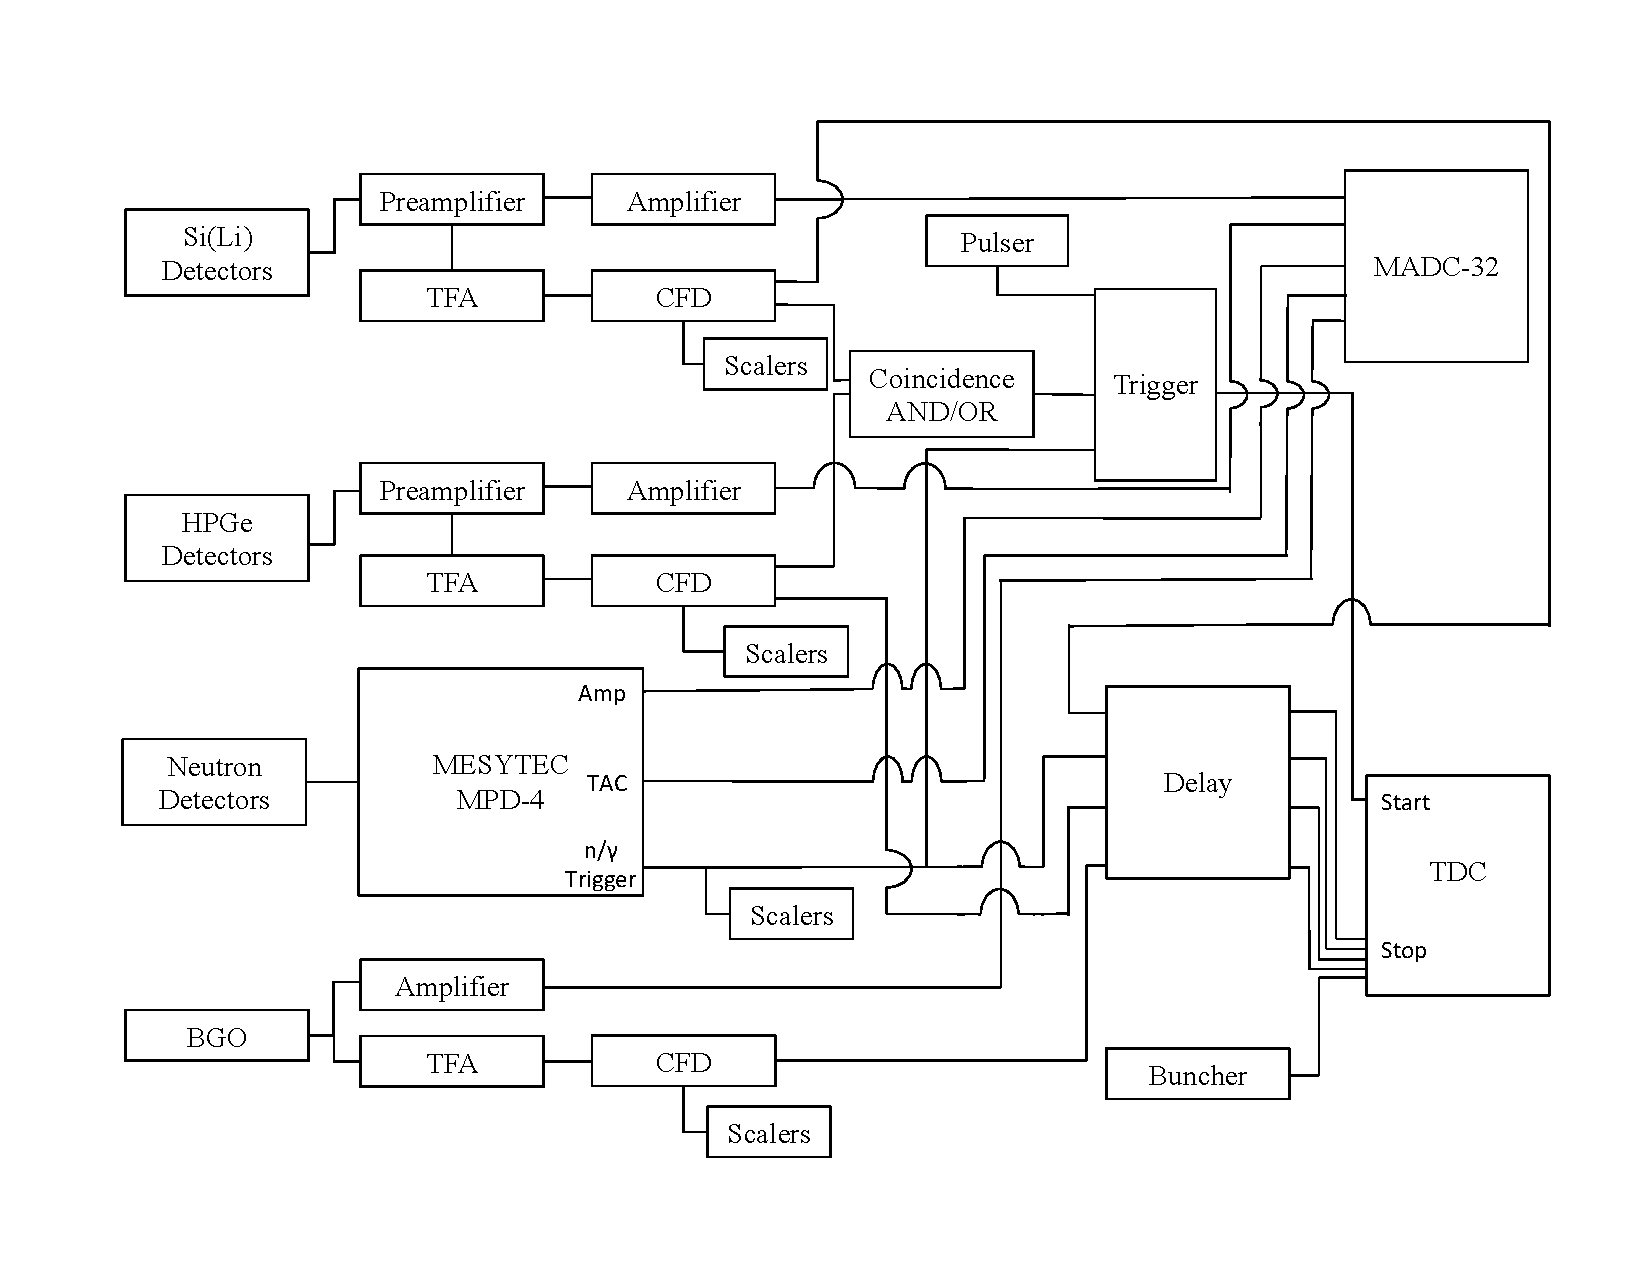
\includegraphics[scale=0.5]{Setup_Figs/electronics-diagram.pdf}
    \caption{A schematic of the electronics for the ICEBall-Georgina set up. See section \ref{sec:GEORGINA_electronics} for a detailed explanation. Taken from \citep{battaglia15:_iceball_176lu}.}
    \label{fig:iceball_electronics}
\end{figure}

The BGO detectors went through an amplifier before being fed directly into the MADC-32. Both the Si(Li)s and the HPGe detectors went into a preamplifier before going into an amplifier, and then the MADC-32. The amplifier allowed for the adjustment of the gain, to optimize the energy regime of interest. The timing signals were sent through a TFA before going through a CFD and being delayed and sent as timing stop signals, as well as being recorded into the scalers. The stop signal was delayed by \~500ns to prevent self-triggering. Start timing signals were put into a logic coincidence for the trigger. The trigger could be adjusted if the count rate were too high, but the ideal case was the "OR" coincidence, where a Si(Li) or HPGe detector could trigger the start. When this occurred, the signal was sent to a trigger, which sent the TDC a start signal. Stop signals could come from any of the three types of detectors, or the bunched beam being used.

The data was collected from the VME modules using the Michigan State University NSCL data acquisition system (DAQ)\citep{nscl:_daq}. The data file, known as an event or "evt" file, is only compatible with the analysis software SpecTcl\citep{nscl:_daq}. For online analysis, SpecTcl was used. However, for the purposes of gating and fitting, it is inadequate. These evt files were instead converted into "root" files, for use with the CERN Root Data Analysis Framework\citep{brun97:_root}. This open source software is programmable through C++, allowing for a robust set of features. This conversion was done using a program called \texttt{evt2root}\citep{smith14:_evt2root}.

\subsection{Clovershare Configuration and Electronics}
\label{sec:clover_electronics}

Due to the fixed nature of the ICEBall detectors, the clovers were limited in the angles they could be placed at to optimize efficiency. With the tungsten blockers in front of the Si(Li) detectors to block gamma-rays and x-rays, placing the clovers behind these detectors would drastically reduce efficiency. The system was modeled in AutoDesk Inventor \citep{autodesk:_inventor} to visualize the detector placement, and find an ideal setup to optimize the HPGe detectors. Figure \ref{fig:inventor} shows the resulting model and placements, as well as several unmoveable obstructions, like cable trays, that needed to be worked around. Figure \ref{fig:clovershare_config} shows the final placements for the seven-detector configuration, in the experimental hall. Table \ref{tab:Clover_Det_Loc} lists the detector placements for the seven and five detector configurations, labeled as Experiments 1 and 2.

\begin{figure}[t]
    \centering
    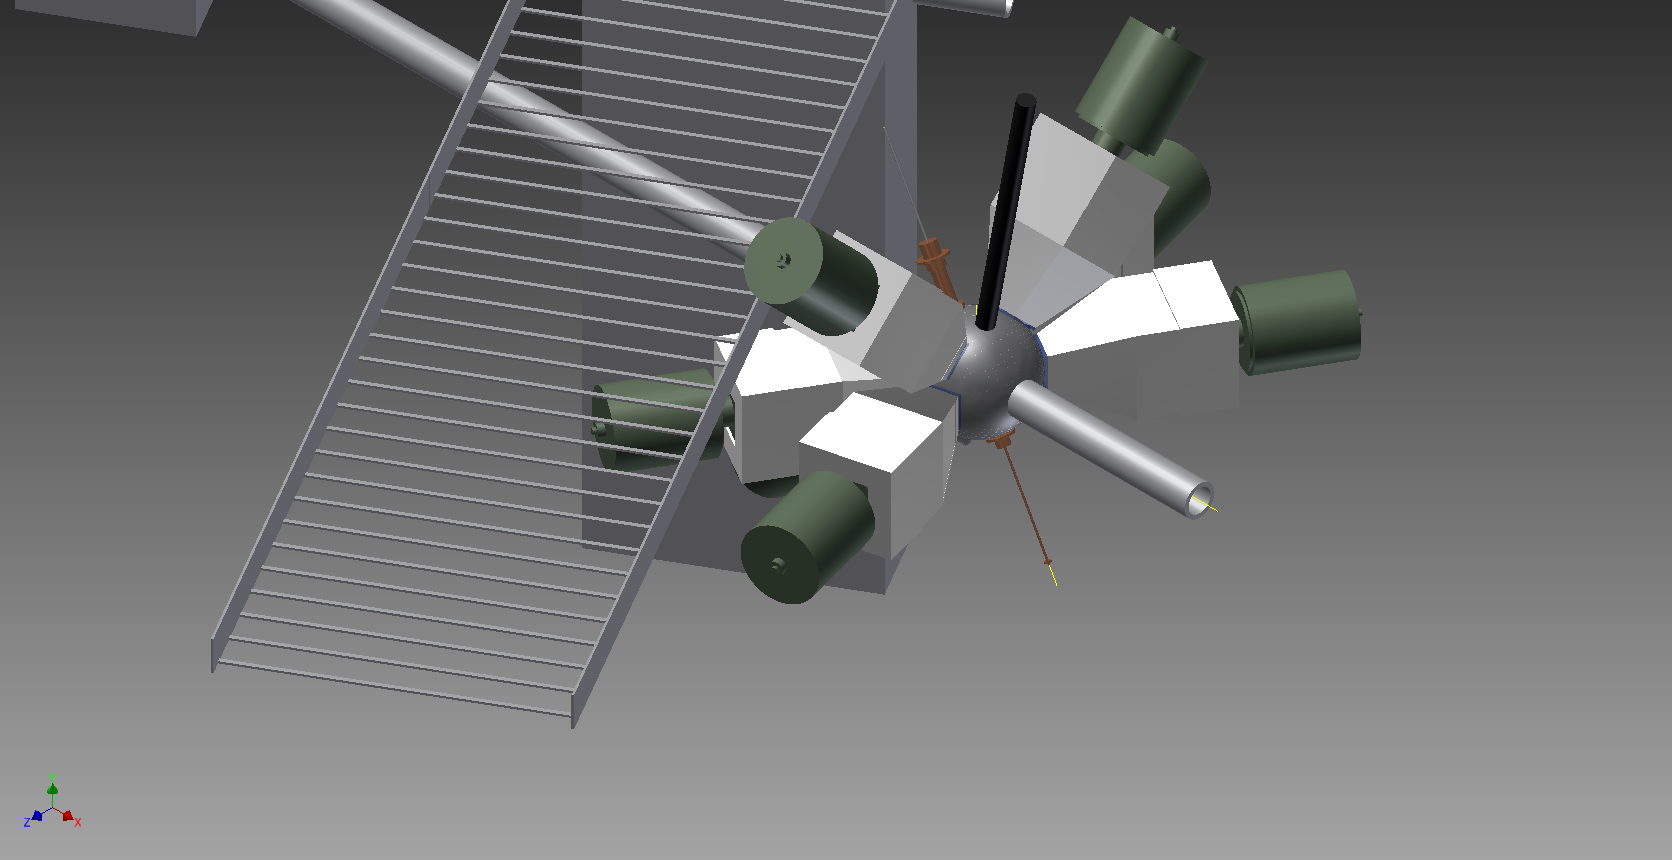
\includegraphics[scale=0.3]{Setup_Figs/FullyAssembled-50cm-newpositions-rightiso.png}
    \caption{ICEBall modeled in Autodesk Inventor \citep{autodesk:_inventor} with the Clovershare detectors placed around it in locations to optimize efficiency. Once ICEBall had been modeled, the detectors were moved around to make sure they were not behind the tungsten blockers. The beamline was also modeled to know where obstructions existed that prevent the Clovershare detectors from being place there.}
    \label{fig:inventor}
\end{figure}

\begin{table}[t]
    \centering
    \caption{Clovershare detector locations}
    \label{tab:Clover_Det_Loc}
    \begin{tabular}{c|c|c!{\vrule width 0.5mm}c|c} \toprule
        & \multicolumn{2}{c!{\vrule width 0.5mm}}{Experiment 1} & \multicolumn{2}{c}{Experiment 2} \\
        \hline
         Detector & $\theta$ & $\phi$ & $\theta$ & $\phi$ \\
         \hline
         ANL-35 & 270 & 145 & 270 & 145 \\ \hline
         LBL-7 & 0 & 111 & 0 & 111 \\ \hline
         ANL-23 & 0 & 66 & \multicolumn{2}{c}{Not Used}\\ \hline
         LBL-6 & 180 & 111 & \multicolumn{2}{c}{Not Used}\\ \hline
         LBL-10 & 180 & 66 & 180 & 71\\ \hline
         ANL-31 & 45 & 90 & 45 & 90\\  \hline
         ANL-18 & 135 & 90 & 180 & 111\\ 
         \bottomrule
    \end{tabular}
    \\[2]
    \footnotesize
    The detectors are listed by identification name. The angles for the detectors are given for both experiments run with the Clovershare detectors. ANL-23 and LBL-6 were not used in the second experiment due to preamplifier issues. The beam axis is the z-axis. $\theta$ is the angle in the xy-plane, where 0 degrees is beam left. $\phi$ is the azimuthal angle, with respect to the beam axis. All values are in degrees.
\end{table}

The electronics used for the Clovershare series of experiments were designed for use with the High Efficiency TOtal absorption spectrometeR (HECTOR), a NaI(Tl) detector array\citep{reingold19:_HECTOR}. The HECTOR data acquisition system is based on the Michigan State University NSCL digital data acquisition system (DDAS). This system uses three XIA Pixie-16 modules \citep{xia:_pixie} which are 16 channel 14-bit 100 MSPS digitizers. The data structure of this system can be seen in Table \ref{tab:word_XIA}. Signals from detectors were fed directly from the preamplifiers to the Pixie modules, which did the amplification, shaping, timing, and logic triggers within the module through adjustments on the data acquisition computer, seen in Figure \ref{fig:pixie_electronics}. In the ICEBall setup, these functions were done using the NIM electronics. NaI(Tl) detectors have far lower resolution than HPGe detectors, so the differential non-linearities are not noticeable in the HECTOR data.

\begin{figure}
    \centering
    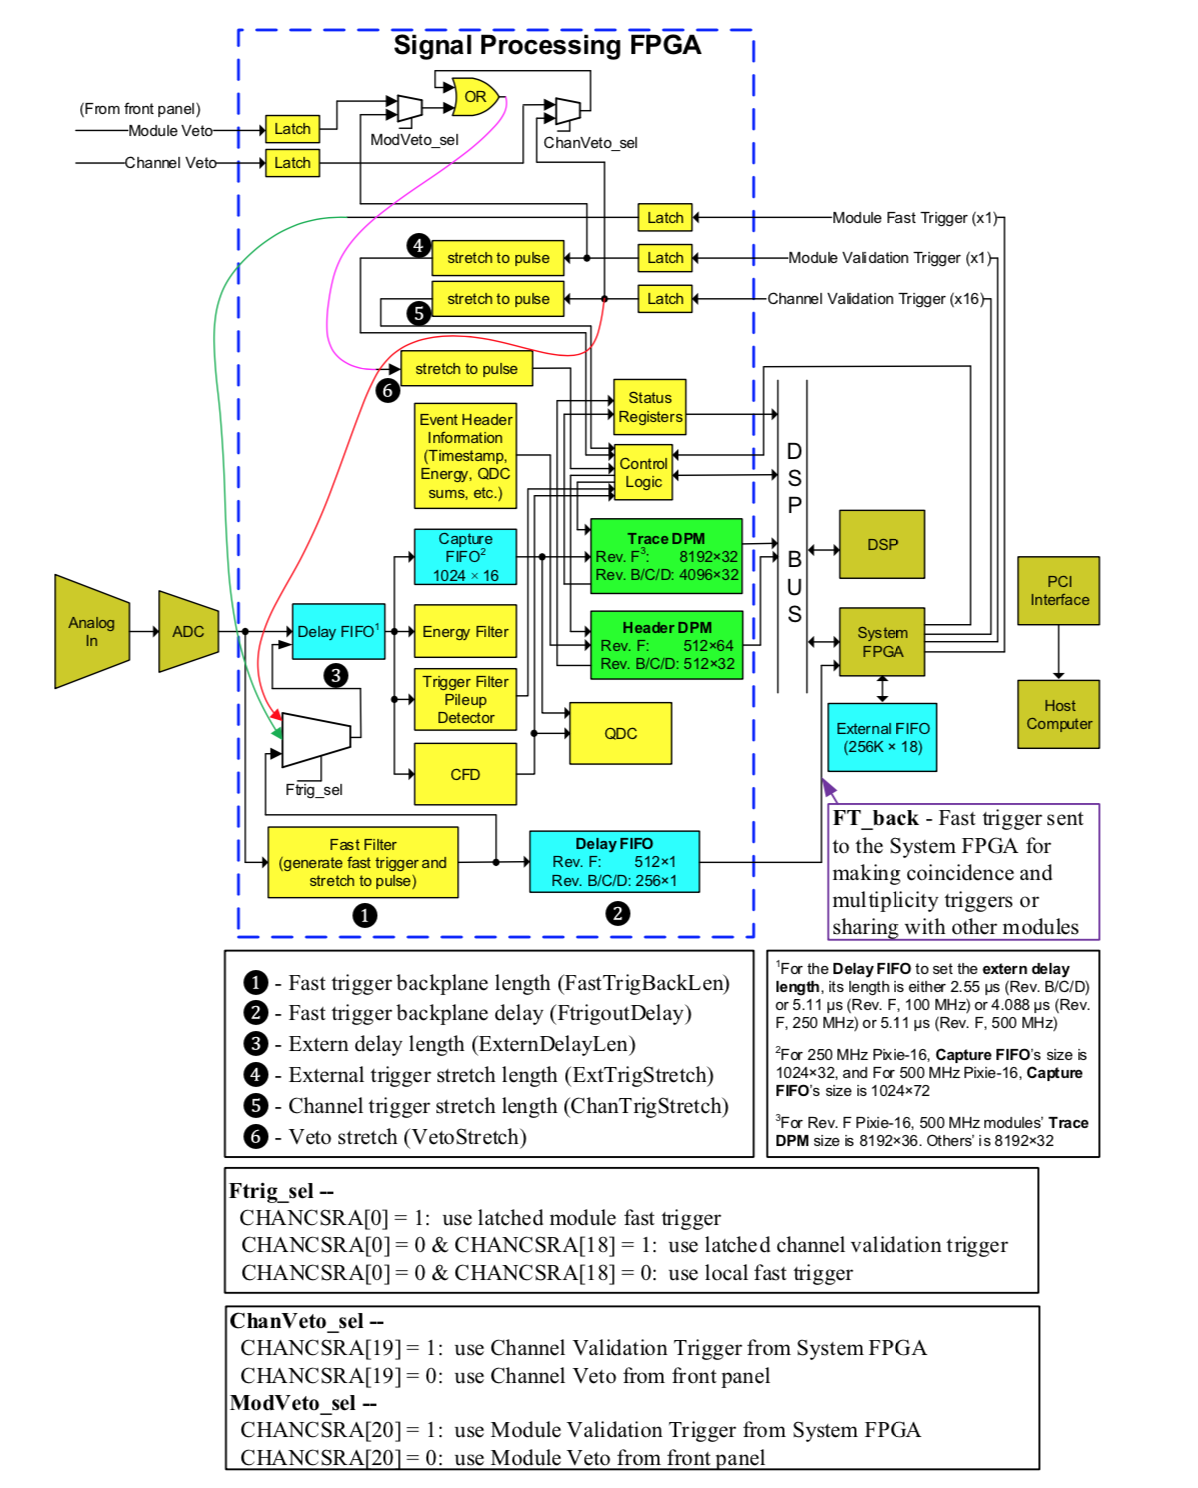
\includegraphics[scale=0.75]{Setup_Figs/pixie_electronics.png}
    \caption{The signal processing done by the XIA Pixie-16 electronics. All the processing is done within the module. Taken from \citep{xia:_pixie}.}
    \label{fig:pixie_electronics}
\end{figure}

The Pixie modules were unable to produce enough gain in the amplifier section for the Si(Li) detectors to cover a significant number of channels for resolution, so the detectors' signals were put through fast filter amplifiers \citep{ortec:_fastamp} to boost the signal before being fed into the DDAS. Fast amplifiers were used due to the fast timing and acquisition nature of the Pixie-16 modules and DDAS. 

As with the ICEBall data, these files were event files that were then converted in root files for further analysis.

\begin{landscape}
\begin{table}[]
    \centering
    \small
    \caption{\label{tab:word_MADC}Data Event - MADC32 (32 Bit Word)}
    \begin{tabular}{c|c|c|c|c|c|c|c|c|c|c|c|c|c|c|c|c|c|c|c|c|c|c|c|c|c|c|c|c|c|c|c}
 %   \begin{tabularx}{\linewidth}{X|X|X|X|X|X|X|X|X|X|X|X|X|X|X|X|X|X|X|X|X|X|X|X|X|X|X|X|X|X|X|X}
        \toprule
        \multicolumn{32}{c}{Header} \\
        \hline
        \multicolumn{2}{c|}{2} & \multicolumn{6}{|c|}{6} & \multicolumn{8}{|c|}{8} & 1 & \multicolumn{3}{|c|}{3} & \multicolumn{2}{|c|}{2} & \multicolumn{10}{|c}{10} \\
        \multicolumn{2}{c|}{header signature} & \multicolumn{6}{|c|}{subheader} & \multicolumn{8}{|c|}{module id} & output format & \multicolumn{3}{|c|}{adc resolution} & \multicolumn{2}{|c|}{} & \multicolumn{10}{|c}{number of data words} \\
        \hline
        \multicolumn{2}{c|}{b01} & \multicolumn{6}{|c|}{b000000} & \multicolumn{8}{|c|}{} & bx & \multicolumn{3}{|c|}{bxxx} & \multicolumn{2}{|c|}{b00} & \multicolumn{10}{|c}{number of 32 bit data words} \\
        \midrule
        \multicolumn{32}{c}{Data Word} \\
        \hline
        \multicolumn{2}{c|}{2} & \multicolumn{9}{|c|}{9} & \multicolumn{5}{|c|}{5} & 1 & 1 & \multicolumn{3}{|c|}{1..3} & \multicolumn{11}{|c}{11..13} \\
        \multicolumn{2}{c|}{data-sig} & \multicolumn{9}{|c|}{} & \multicolumn{5}{|c|}{} &  & out of range & \multicolumn{3}{|c|}{} & \multicolumn{11}{|c}{} \\
        \hline
        \multicolumn{2}{c|}{b00} & \multicolumn{9}{|c|}{00 0100 000} & \multicolumn{5}{|c|}{channel number} & b0  & Oor & \multicolumn{3}{|c|}{b00} & \multicolumn{11}{|c}{ADC Amplitude} \\
        \midrule
        \multicolumn{32}{c}{End of Event} \\
        \hline
        \multicolumn{2}{c|}{2} & \multicolumn{30}{|c}{30} \\
        \hline
        \multicolumn{2}{c|}{b11} & \multicolumn{30}{|c}{event counter/time stamp} \\
        \bottomrule
    \end{tabular}
    \\[2pt]
    \footnotesize
    Table of the 32-bit word data structure of the MADC. The headers, event word structure, and end of event structure, where needed, are all listed. In the tables, the first row in a given block is the number of bits used by that piece of data, while the second row is a description of the data. Bits go in descending order from left to right.
    \end{table}
    
    \pagebreak
    
    \begin{table}[]
    \centering
    \caption{\label{tab:word_CAEN}Data Event - V775 (32 Bit Word)}
    \begin{tabular}{c|c|c|c|c|c|c|c|c|c|c|c|c|c|c|c|c|c|c|c|c|c|c|c|c|c|c|c|c|c|c|c}
        \toprule
        \multicolumn{32}{c}{Header} \\
        \hline
        \multicolumn{5}{c|}{5} & \multicolumn{3}{|c|}{3} & \multicolumn{8}{|c|}{8} & \multicolumn{2}{|c|}{2} & \multicolumn{6}{|c|}{6} & \multicolumn{8}{|c}{8} \\
        \hline
        \multicolumn{5}{c|}{Geo Address[5]} & \multicolumn{3}{|c|}{010} & \multicolumn{8}{|c|}{Crate Number[8]} & \multicolumn{2}{|c|}{00} & \multicolumn{6}{|c|}{Converted Channels[6]} & \multicolumn{8}{|c}{} \\
        \midrule
        \multicolumn{32}{c}{Data Word} \\
        \hline
        \multicolumn{5}{c|}{5} & \multicolumn{3}{|c|}{3} & \multicolumn{3}{|c|}{3} & \multicolumn{5}{|c|}{5} & 1 & 1 & 1 & 1 & \multicolumn{12}{|c}{12}\\
        \hline
        \multicolumn{5}{c|}{Geo Address[5]} & \multicolumn{3}{|c|}{000} & \multicolumn{3}{|c|}{} & \multicolumn{5}{|c|}{Channel Number} &  & Valid & Under-Threshold & Overflow & \multicolumn{12}{|c}{ADC Amplitude[12]}\\
        \midrule
        \multicolumn{32}{c}{End of Block} \\
        \hline
        \multicolumn{5}{c|}{5} & \multicolumn{3}{|c|}{3} & \multicolumn{24}{|c}{24} \\
        \hline
        \multicolumn{5}{c|}{Geo Address[5]} & \multicolumn{3}{|c|}{100} & \multicolumn{24}{|c}{Event Counter[24]} \\
        \bottomrule
    \end{tabular}
    \\[2pt]
    \footnotesize
    Table of the 32-bit word data structure of the CAEN 775 TDC. The headers, event word structure, and end of event structure, where needed, are all listed. In the tables, the first row in a given block is the number of bits used by that piece of data, while the second row is a description of the data. Bits go in descending order from left to right.
    \end{table}

    \pagebreak
    
    \begin{table}[]
    \small
    \centering
    \caption{\label{tab:word_V830}Data Event - V830 (32 Bit Word)}
    \begin{tabular}{c|c|c|c|c|c|c|c|c|c|c|c|c|c|c|c|c|c|c|c|c|c|c|c|c|c|c|c|c|c|c|c|c}
        \toprule
        \multicolumn{32}{c}{Header} \\
        \hline
        \multicolumn{5}{c|}{5} & 1 & \multicolumn{2}{|c|}{2} & \multicolumn{6}{|c|}{6} & \multicolumn{2}{|c|}{2} & \multicolumn{16}{|c|}{16}\\
        \hline
        \multicolumn{5}{c|}{Geo Address} & 1 & \multicolumn{2}{|c|}{} & \multicolumn{6}{|c|}{Number of} & \multicolumn{2}{|c|}{Source} & \multicolumn{16}{|c|}{Trigger}\\
        \addlinespace[-2ex]
        \multicolumn{5}{c|}{Geo Address} & 1 & \multicolumn{2}{|c|}{} & \multicolumn{6}{|c|}{Enabled Channels} & \multicolumn{2}{|c|}{Source} & \multicolumn{16}{|c|}{Number}\\
        \midrule
        \multicolumn{32}{c}{Data Word} \\
        \hline
         \multicolumn{32}{c}{32} \\
        \hline
         \multicolumn{32}{c}{Channel Counter[32]} \\
        \bottomrule
    \end{tabular}
    \\[2pt]
    \footnotesize
    Table of the 32-bit word data structure of the CAEN V830 Scaler. The headers, event word structure, and end of event structure, where needed, are all listed. In the tables, the first row in a given block is the number of bits used by that piece of data, while the second row is a description of the data. Bits go in descending order from left to right.
\end{table}
    
    \pagebreak
    
    \begin{table}[]
    \small
    \centering
    \caption{\label{tab:word_XIA}Data Event - Pixie-16 (32 Bit Word)}
    \begin{tabular}{c|c|c|c|c|c|c|c|c|c|c|c|c|c|c|c|c|c|c|c|c|c|c|c|c|c|c|c|c|c|c|c|c}
    \toprule
        Index & \multicolumn{32}{|c}{Header}\\
        \midrule
        \multirow{2}{*}{0} & 1 & \multicolumn{14}{|c|}{14} & \multicolumn{5}{|c|}{5} & \multicolumn{4}{|c|}{4} & \multicolumn{4}{|c|}{4} & \multicolumn{4}{|c}{4} \\
        \cline{2-33}
        & Finish Code & \multicolumn{14}{|c|}{Event Length} & \multicolumn{5}{|c|}{Header Length} & \multicolumn{4}{|c|}{CrateID} & \multicolumn{4}{|c|}{SlotID} & \multicolumn{4}{|c}{Chan\#} \\
        \midrule
        \multirow{2}{*}{1} & \multicolumn{32}{|c}{32} \\
        \cline{2-33}
        & \multicolumn{32}{|c}{EVTTIME\_LO[32]} \\
        \midrule
        \multirow{2}{*}{2} & 1 & \multicolumn{15}{|c|}{15} & \multicolumn{16}{|c}{16}\\
        \cline{2-33}
        & CFD forced trigger bit & \multicolumn{15}{|c|}{CFD Fractional Time[15] x 32768} & \multicolumn{16}{|c}{EVTTIME\_HI[16]} \\
        \midrule
        \multirow{2}{*}{3} & 1 & \multicolumn{15}{|c|}{15} & \multicolumn{16}{|c}{16}\\
        \cline{2-33}
        & Trace Out-of-Range Flag & \multicolumn{15}{|c|}{Trace Length} & \multicolumn{16}{|c}{Event Energy}\\
        \midrule
        \multicolumn{33}{c}{Data Word} \\
        \midrule
        \multirow{2}{*}{n} & \multicolumn{16}{|c|}{16} & \multicolumn{16}{|c}{16} \\
        \cline{2-33}
        & \multicolumn{16}{|c|}{ADC Data \#(2n+1)[16]} & \multicolumn{16}{|c}{ADC Data \#(2n)[16]} \\
        \bottomrule
    \end{tabular}
    \\[2pt]
    \footnotesize
    Table of the 32-bit word data structure of the Xia Pixie-16. The headers, event word structure, and end of event structure, where needed, are all listed. In the tables, the first row in a given block is the number of bits used by that piece of data, while the second row is a description of the data. Bits go in descending order from left to right.
\end{table}
\end{landscape}